\chapter{The Appendices for Experiment}\label{app:Exp}
\section{Mass resolution fit results}
\label{app:_mas_res}
As described in \ref{sec:mass_res}, for 2017 the quantity $\frac{(M_{reco} - M_{gen})}{M_{gen}}$ is fitted in bins of $M_{gen}$ using a double-sided crystal ball (dCB) function. The fits results are shown for the different mass points in fig. \ref{fig:fit_BB} for the Barrel-Barrel category (BB) and in fig. \ref{fig:fit_BE} for the Barrel-Endcap (BE) category.
\begin{figure}[ht]
  \begin{center}
    \begin{tabular}{cccc}
      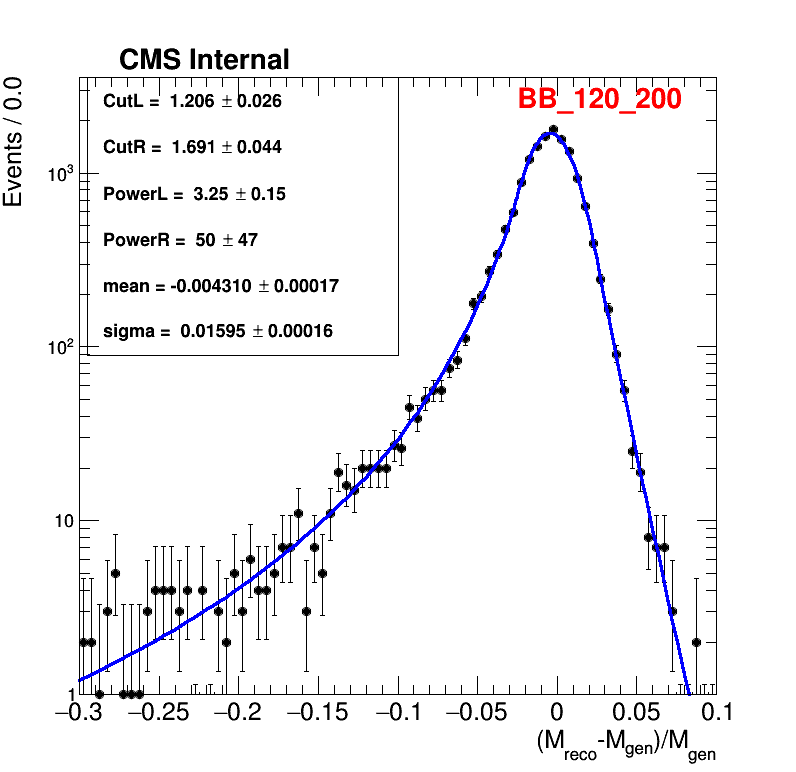
\includegraphics[width=0.22\textwidth]{figures/Zprime/2017/mass_resolution/High_Mass/BB_120_200} &
      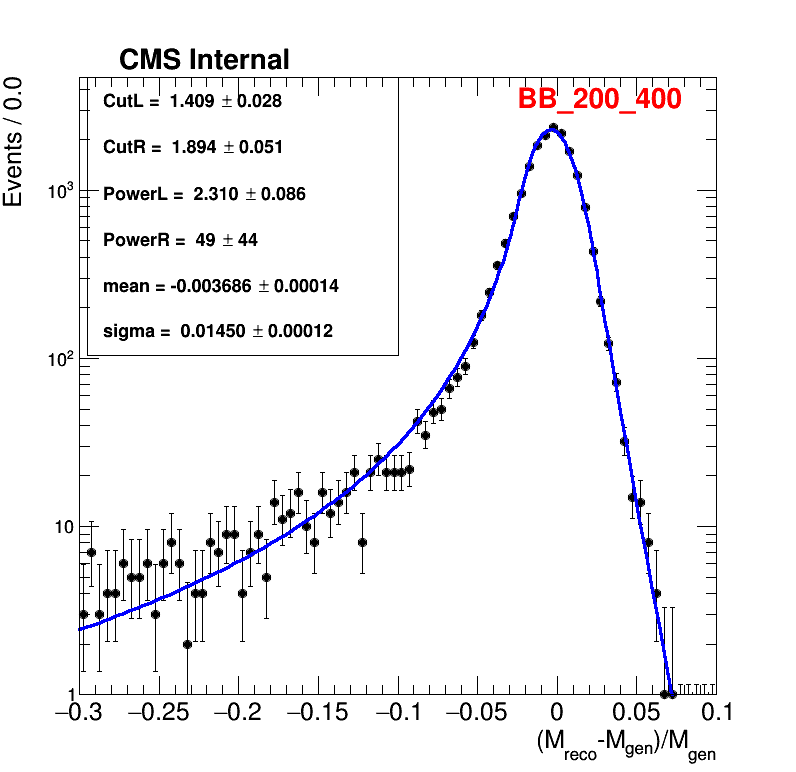
\includegraphics[width=0.22\textwidth]{figures/Zprime/2017/mass_resolution/High_Mass/BB_200_400}&
      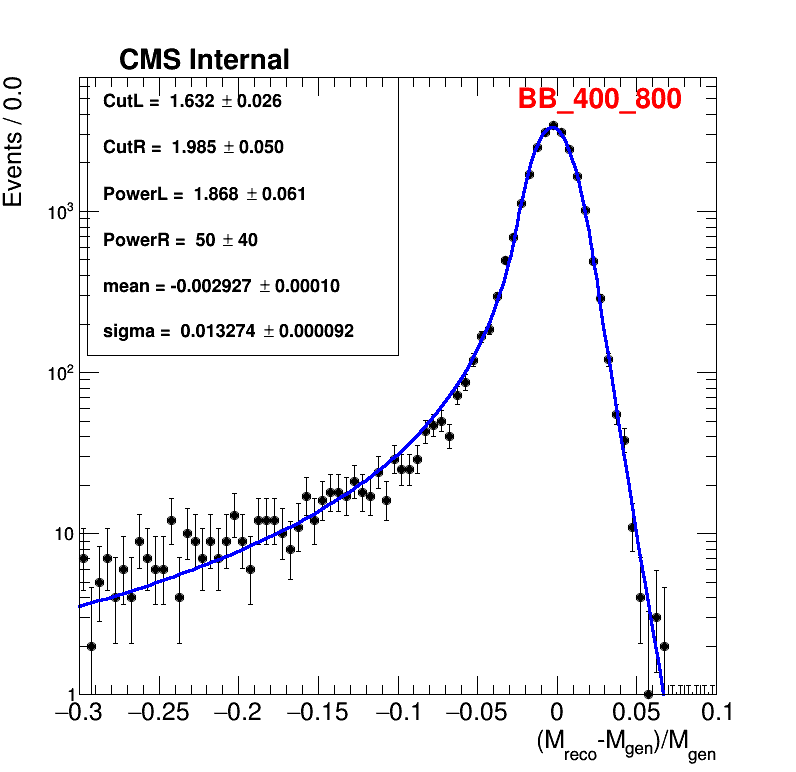
\includegraphics[width=0.22\textwidth]{figures/Zprime/2017/mass_resolution/High_Mass/BB_400_800} &
      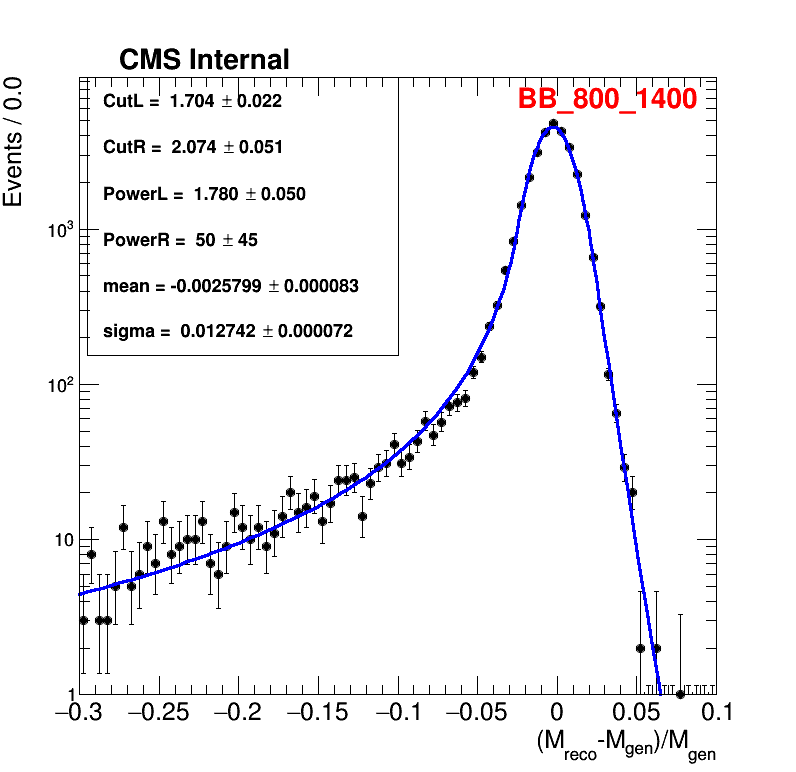
\includegraphics[width=0.22\textwidth]{figures/Zprime/2017/mass_resolution/High_Mass/BB_800_1400} \\
      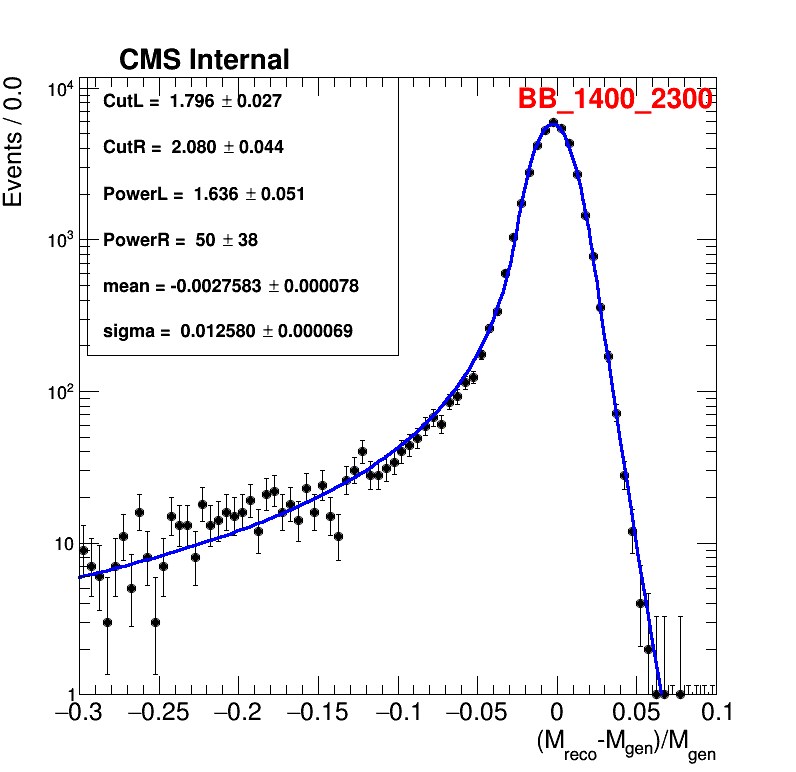
\includegraphics[width=0.22\textwidth]{figures/Zprime/2017/mass_resolution/High_Mass/BB_1400_2300}&
      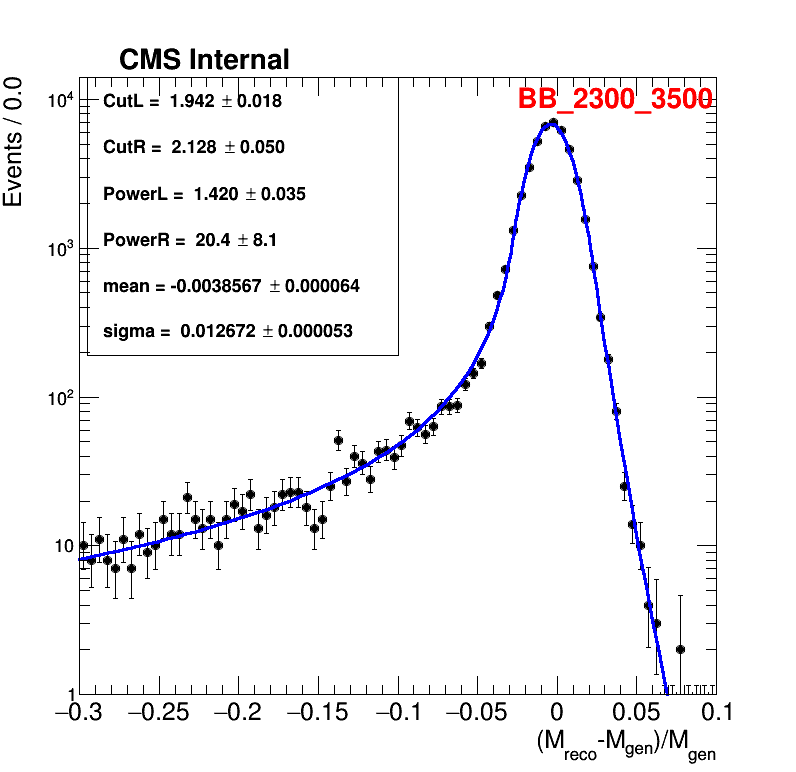
\includegraphics[width=0.22\textwidth]{figures/Zprime/2017/mass_resolution/High_Mass/BB_2300_3500}&
      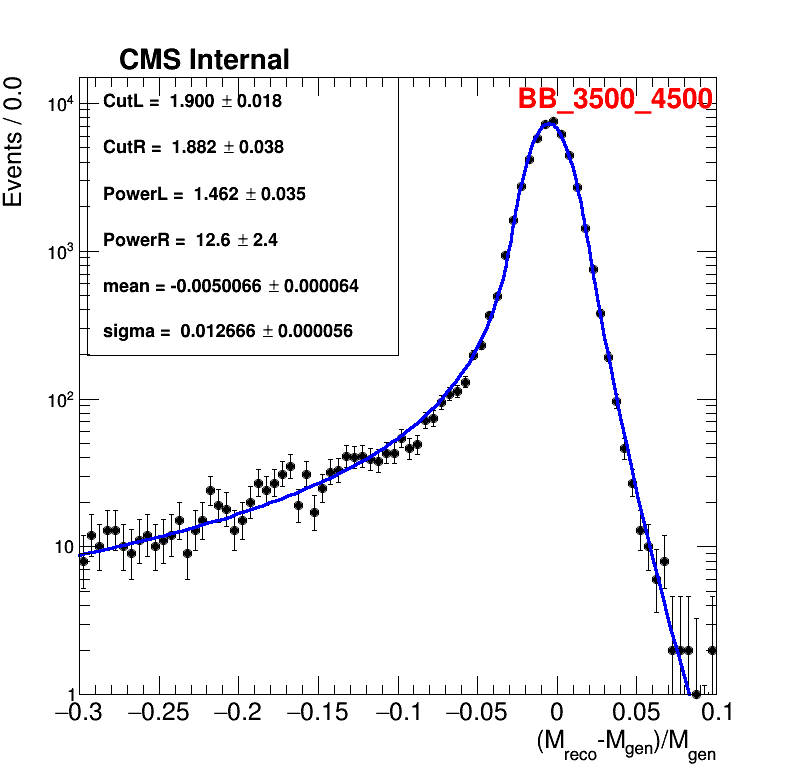
\includegraphics[width=0.22\textwidth]{figures/Zprime/2017/mass_resolution/High_Mass/BB_3500_4500}&
      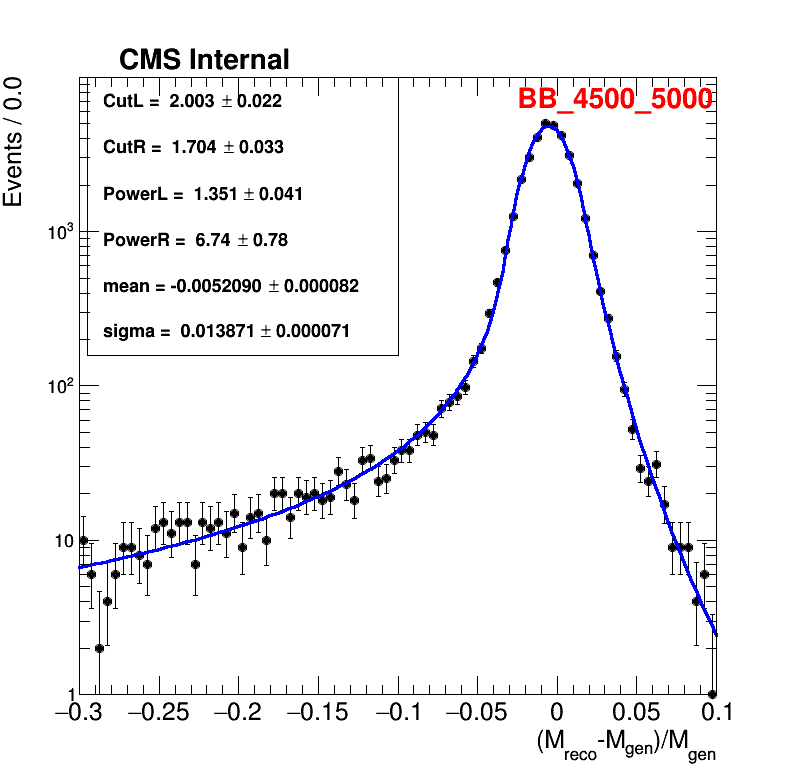
\includegraphics[width=0.22\textwidth]{figures/Zprime/2017/mass_resolution/High_Mass/BB_4500_5000}\\
    \end{tabular}
    \caption{Fit results of the $\frac{(M_{reco} - M_{gen})}{M_{gen}}$ histograms in the BB category per $M_{gen}$ bins.
    \label{fig:fit_BB}}
  \end{center}
\end{figure}

\begin{figure}[ht]
  \begin{center}
    \begin{tabular}{cccc}
      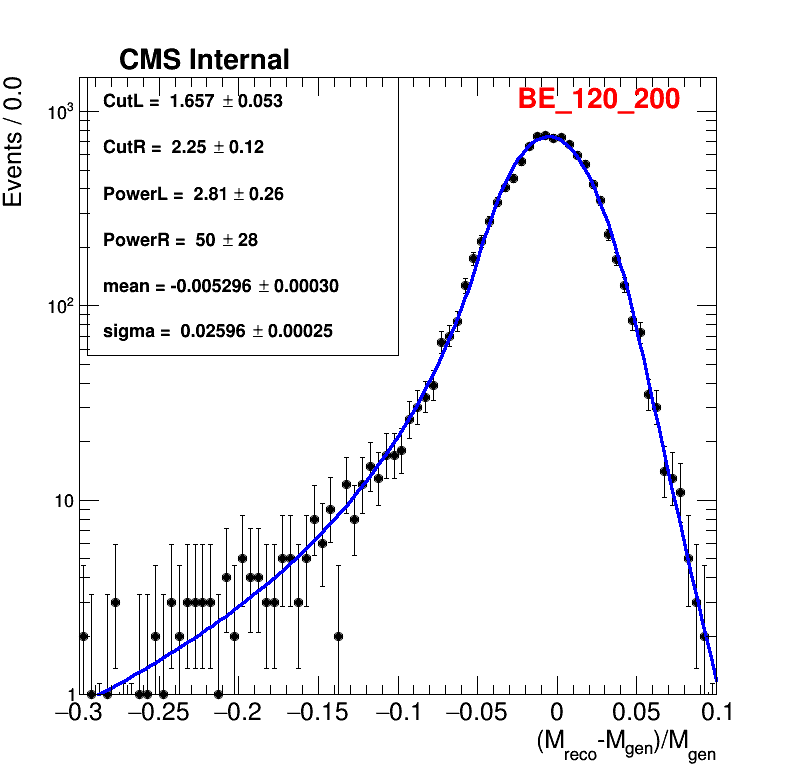
\includegraphics[width=0.22\textwidth]{figures/Zprime/2017/mass_resolution/High_Mass/BE_120_200} &
      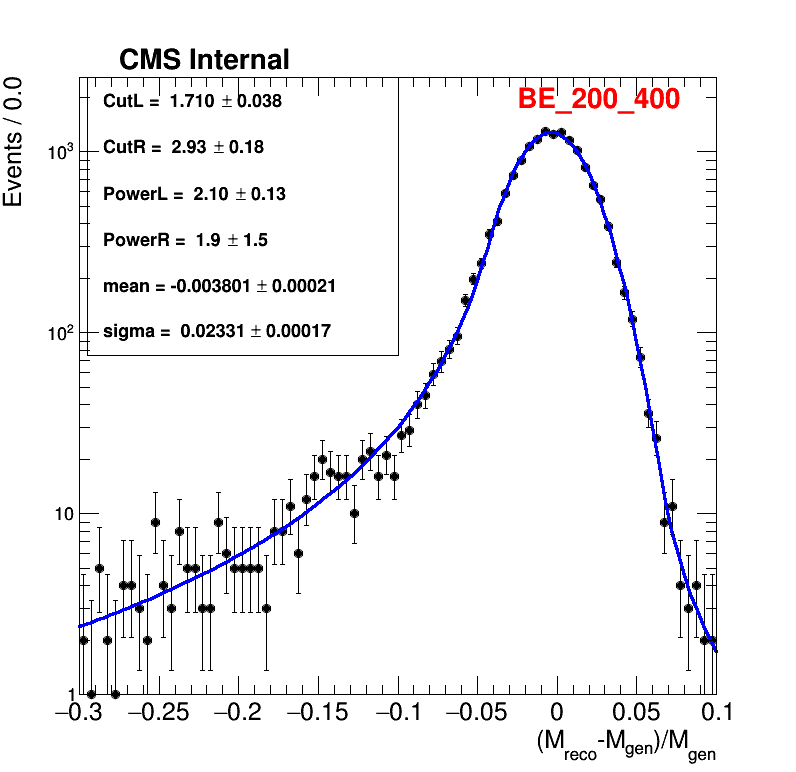
\includegraphics[width=0.22\textwidth]{figures/Zprime/2017/mass_resolution/High_Mass/BE_200_400}&
      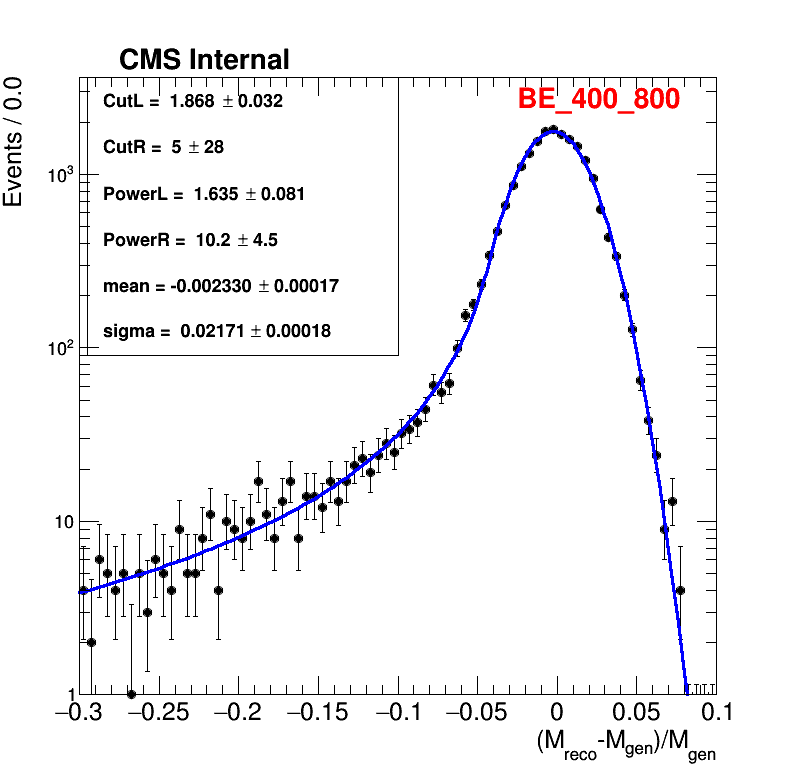
\includegraphics[width=0.22\textwidth]{figures/Zprime/2017/mass_resolution/High_Mass/BE_400_800} &
      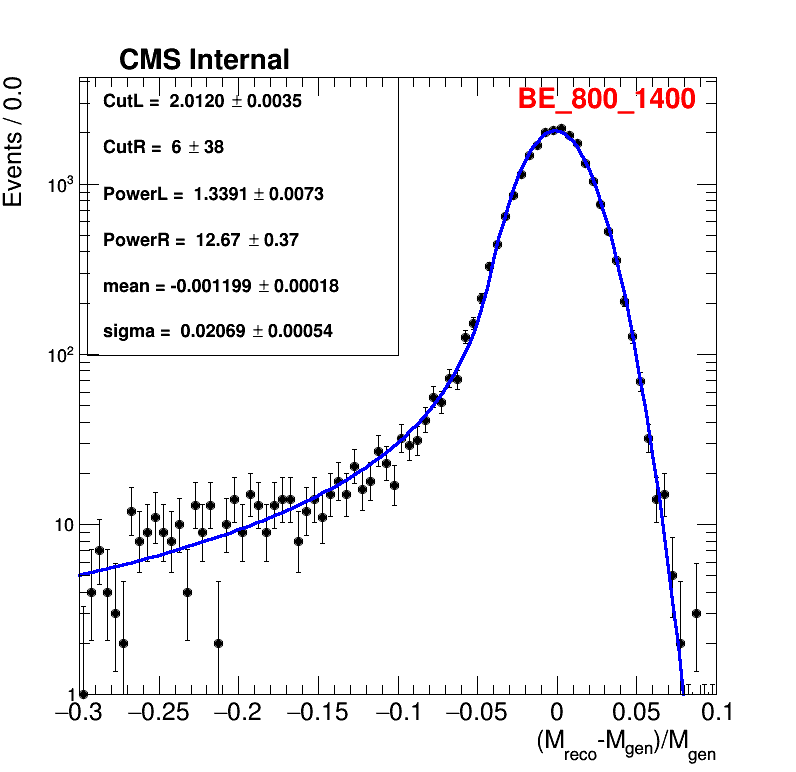
\includegraphics[width=0.22\textwidth]{figures/Zprime/2017/mass_resolution/High_Mass/BE_800_1400} \\
      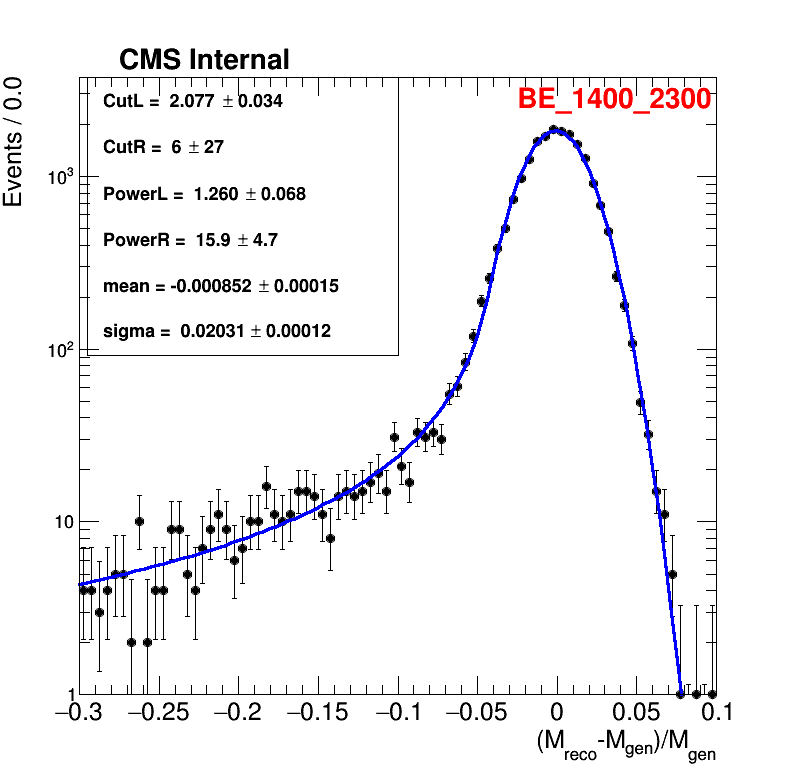
\includegraphics[width=0.22\textwidth]{figures/Zprime/2017/mass_resolution/High_Mass/BE_1400_2300} &
      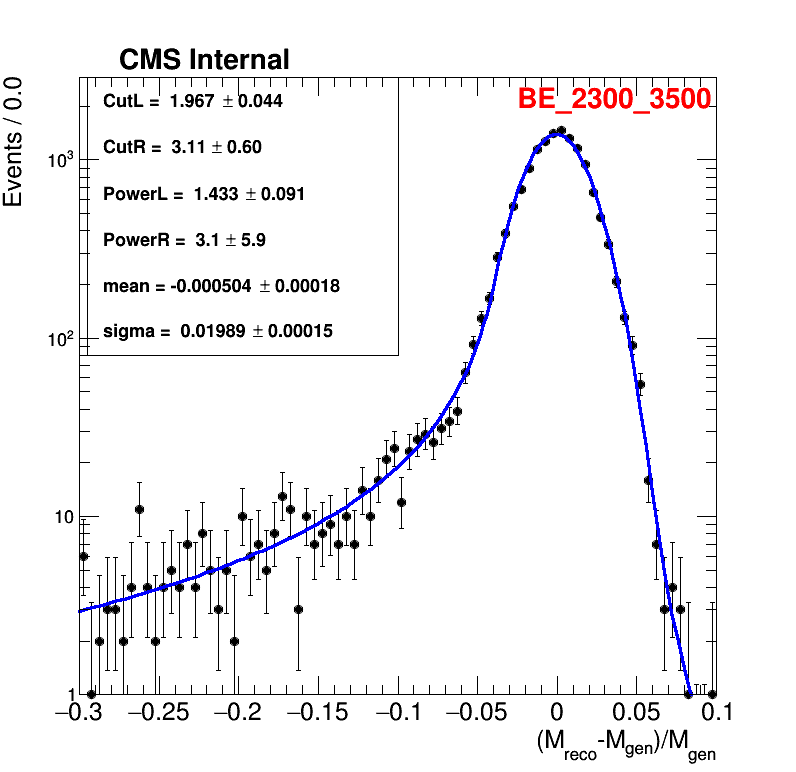
\includegraphics[width=0.22\textwidth]{figures/Zprime/2017/mass_resolution/High_Mass/BE_2300_3500}&
      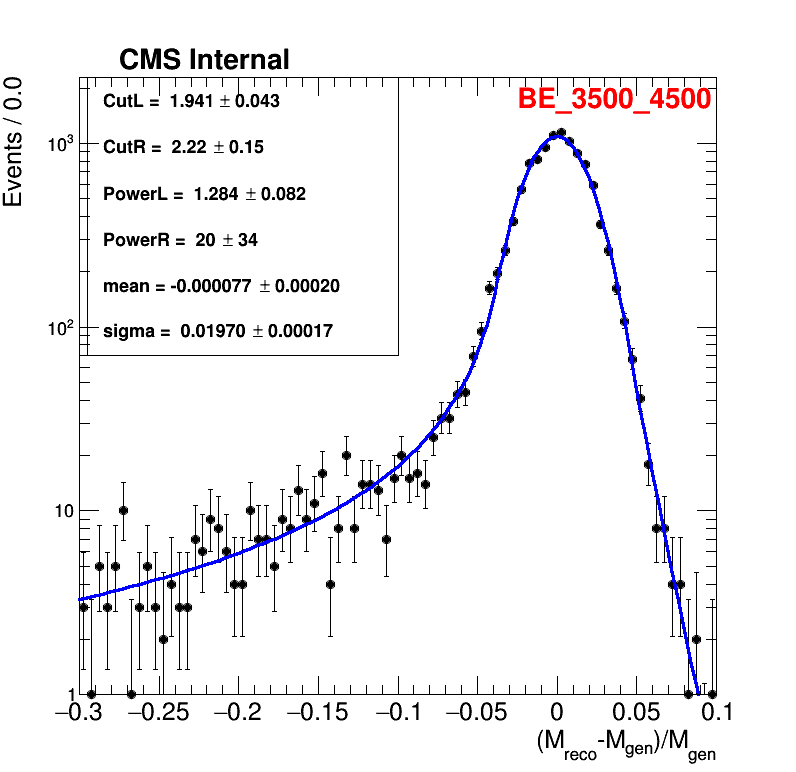
\includegraphics[width=0.22\textwidth]{figures/Zprime/2017/mass_resolution/High_Mass/BE_3500_4500} &
      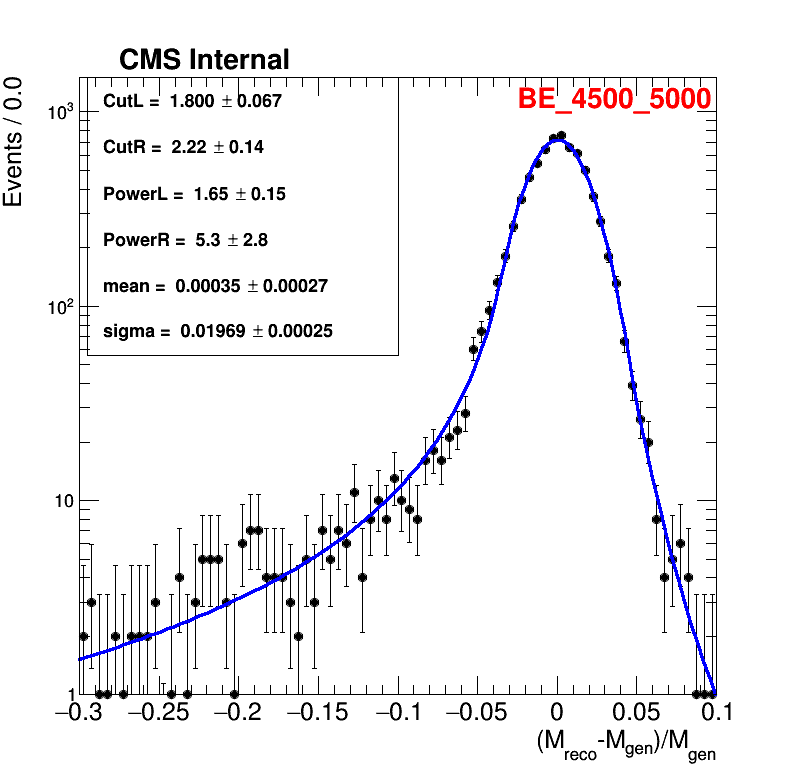
\includegraphics[width=0.22\textwidth]{figures/Zprime/2017/mass_resolution/High_Mass/BE_4500_5000}\\
    \end{tabular}
    \caption{Fit results of the $\frac{(M_{reco} - M_{gen})}{M_{gen}}$ histograms in the BE category per $M_{gen}$ bins.
    \label{fig:fit_BE}}
  \end{center}
\end{figure}

The parameters of the fitted dCB functions are then drawn as functions of $M_{gen}$ and a fit is superimposed in order to get an analytic description of their behaviour (see fig. \ref{fig:fit_parameters_BB} and \ref{fig:fit_parameters_BE} ).

\begin{figure}[ht]
  \begin{center}
    \begin{tabular}{cccc}
      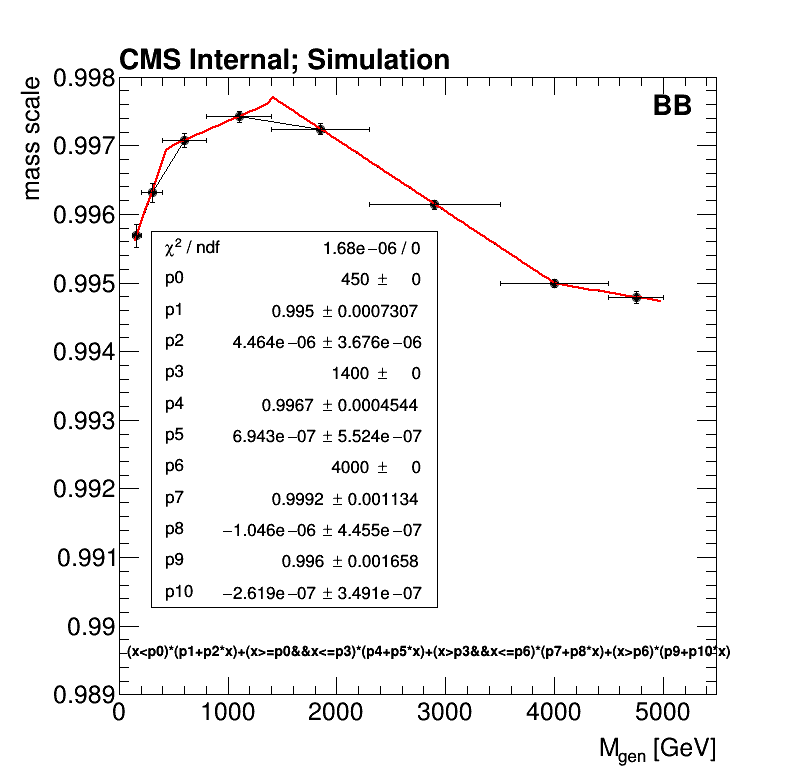
\includegraphics[width=0.45\textwidth]{figures/Zprime/2017/mass_resolution/High_Mass/BB_mean} &
      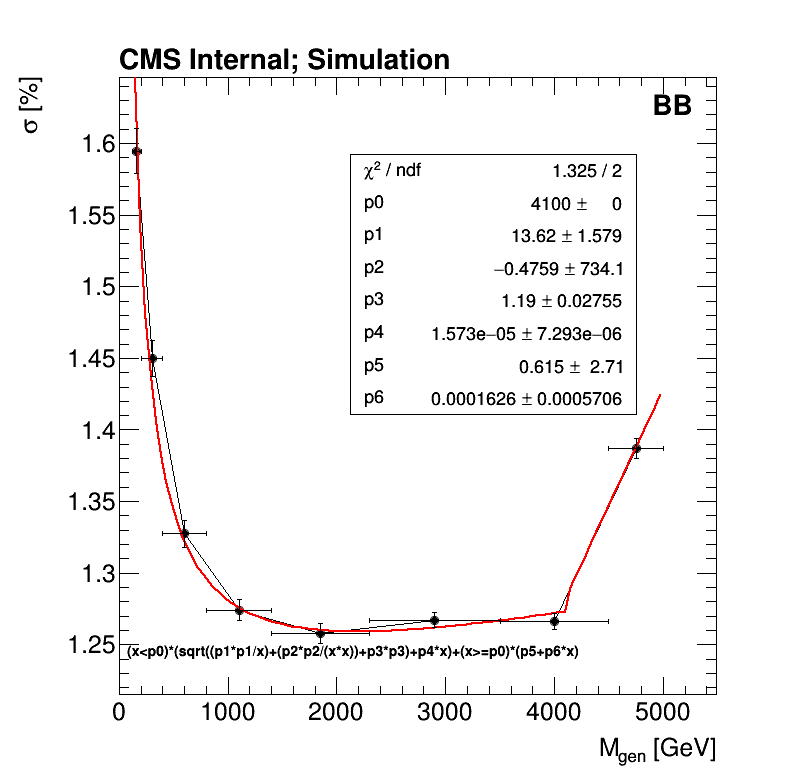
\includegraphics[width=0.45\textwidth]{figures/Zprime/2017/mass_resolution/High_Mass/BB_sigma}\\
      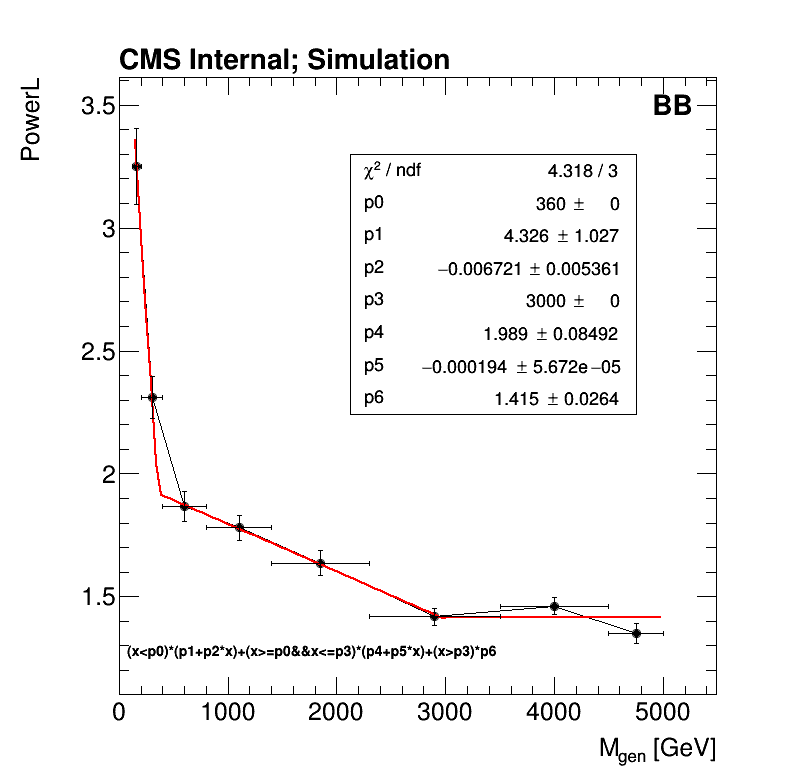
\includegraphics[width=0.45\textwidth]{figures/Zprime/2017/mass_resolution/High_Mass/BB_PowerL} &
      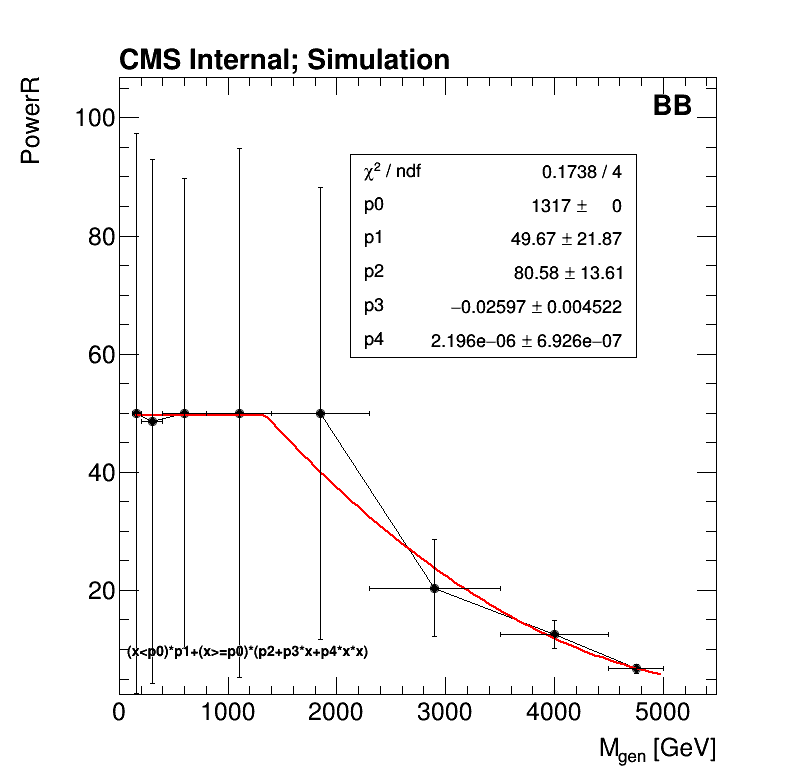
\includegraphics[width=0.45\textwidth]{figures/Zprime/2017/mass_resolution/High_Mass/BB_PowerR} \\
      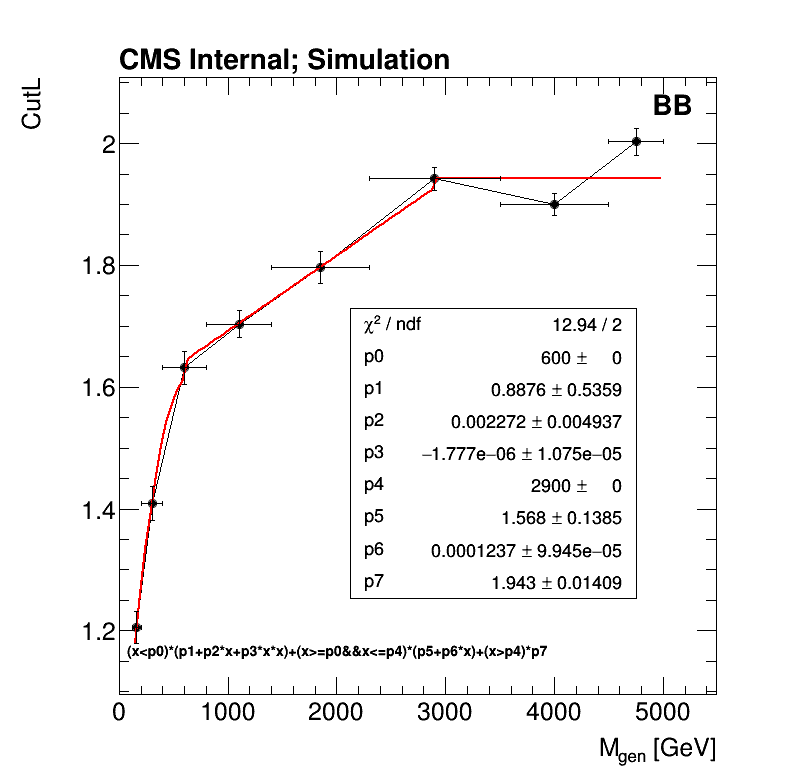
\includegraphics[width=0.45\textwidth]{figures/Zprime/2017/mass_resolution/High_Mass/BB_CutL} &
      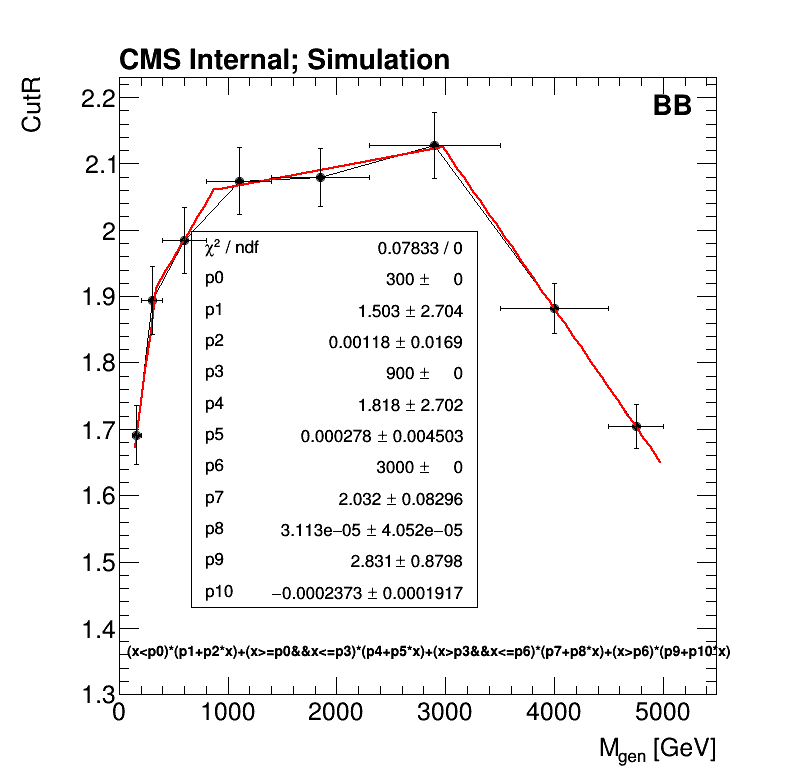
\includegraphics[width=0.45\textwidth]{figures/Zprime/2017/mass_resolution/High_Mass/BB_CutR} \\
    \end{tabular}
    \caption{Parameters of the dCB as a function of $M_{gen}$ for BB category.
    \label{fig:fit_parameters_BB}}
  \end{center}
\end{figure}

\begin{figure}[ht]
  \begin{center}
    \begin{tabular}{cccc}
      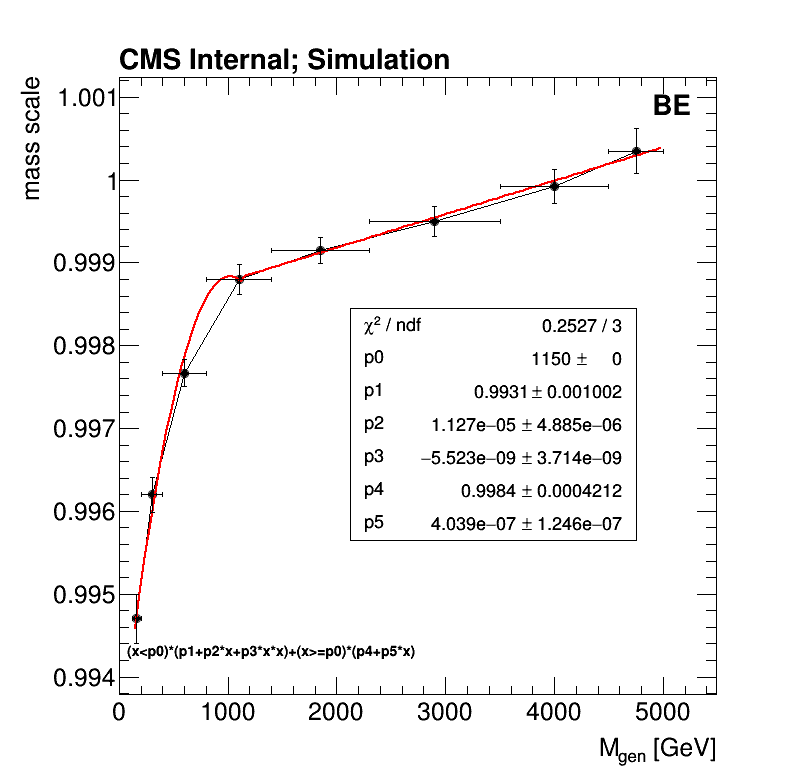
\includegraphics[width=0.45\textwidth]{figures/Zprime/2017/mass_resolution/High_Mass/BE_mean} &
      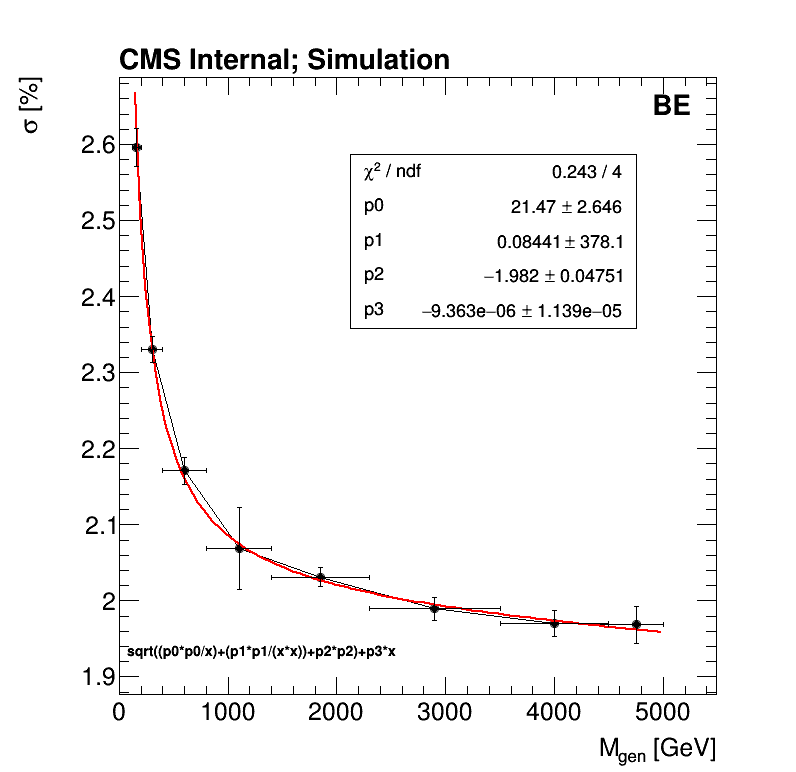
\includegraphics[width=0.45\textwidth]{figures/Zprime/2017/mass_resolution/High_Mass/BE_sigma}\\
      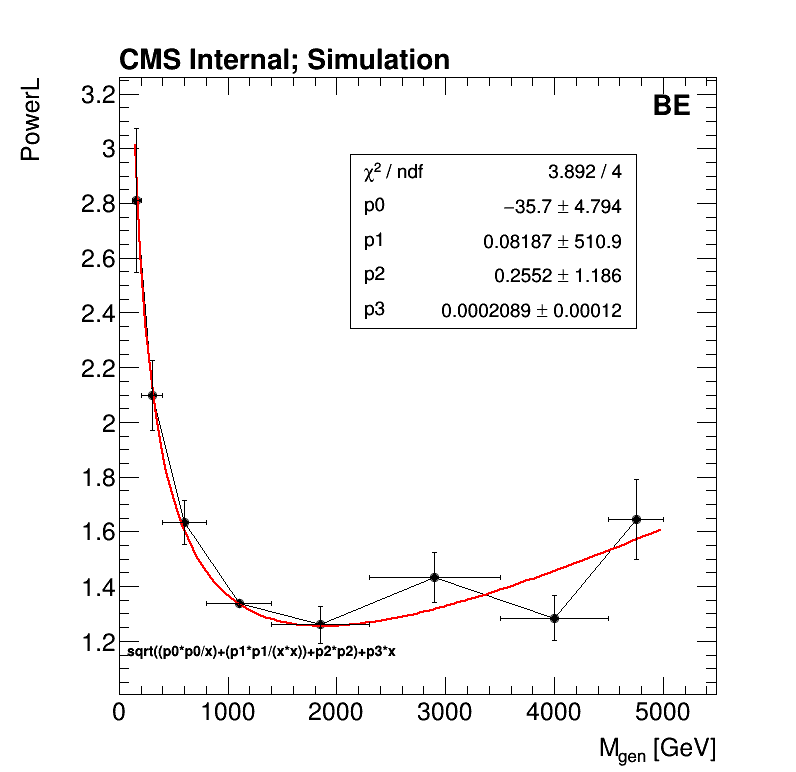
\includegraphics[width=0.45\textwidth]{figures/Zprime/2017/mass_resolution/High_Mass/BE_PowerL} &
      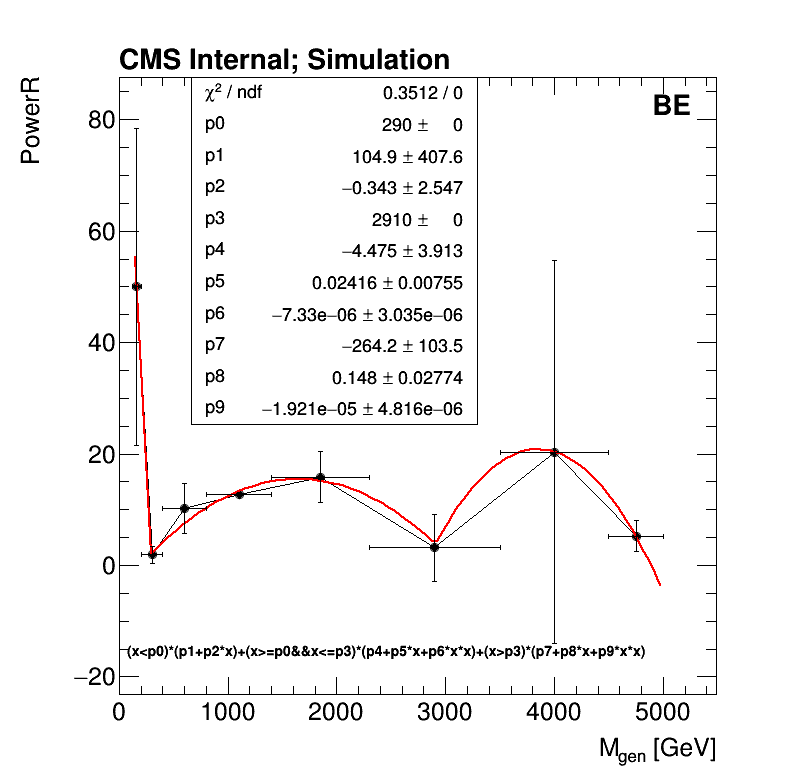
\includegraphics[width=0.45\textwidth]{figures/Zprime/2017/mass_resolution/High_Mass/BE_PowerR} \\
      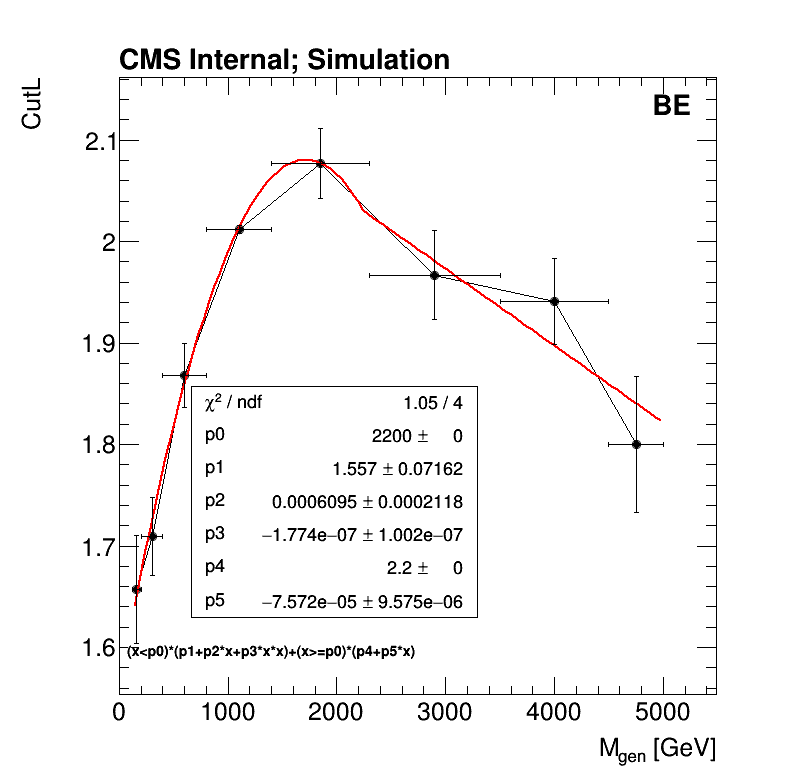
\includegraphics[width=0.45\textwidth]{figures/Zprime/2017/mass_resolution/High_Mass/BE_CutL} &
      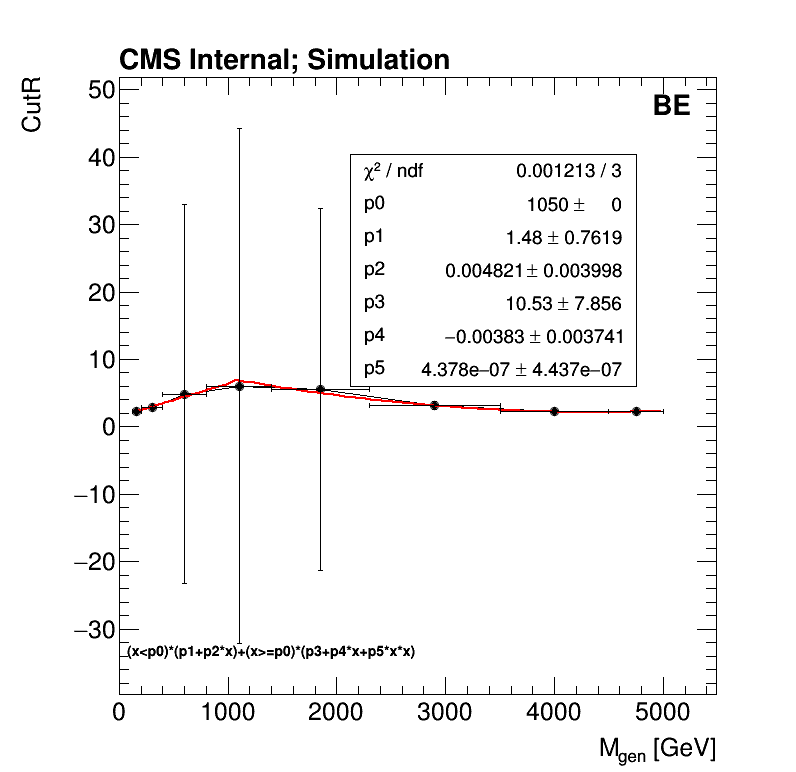
\includegraphics[width=0.45\textwidth]{figures/Zprime/2017/mass_resolution/High_Mass/BE_CutR} \\
    \end{tabular}
    \caption{Parameters of the dCB as a function of $M_{gen}$ for BE category.
    \label{fig:fit_parameters_BE}}
  \end{center}
\end{figure}

At this point, in the limit setting procedure, the mass resolution is treated as a dCB function whose parameters are described by the analytic functions derived from \ref{fig:fit_parameters_BB} and \ref{fig:fit_parameters_BE}.

%Finally, as a closure test of the procedure, the $\frac{(M_{reco} - M_{gen})}{M_{gen}}$ histograms are plotted superimposing the RC function that is used for the limit setting procedure, finding of good level of agreement for all the $M_{gen}$ bins. The only bins where the agreement is not optimal are the first two (upper left in fig. \ref{fig:fit_closure_BB} and \ref{fig:fit_closure_BE}) which correspond to $M_{gen}< $150 GeV, below the searching region.
%\begin{figure}[ht]
%  \begin{center}
%    \begin{tabular}{cccc}
%      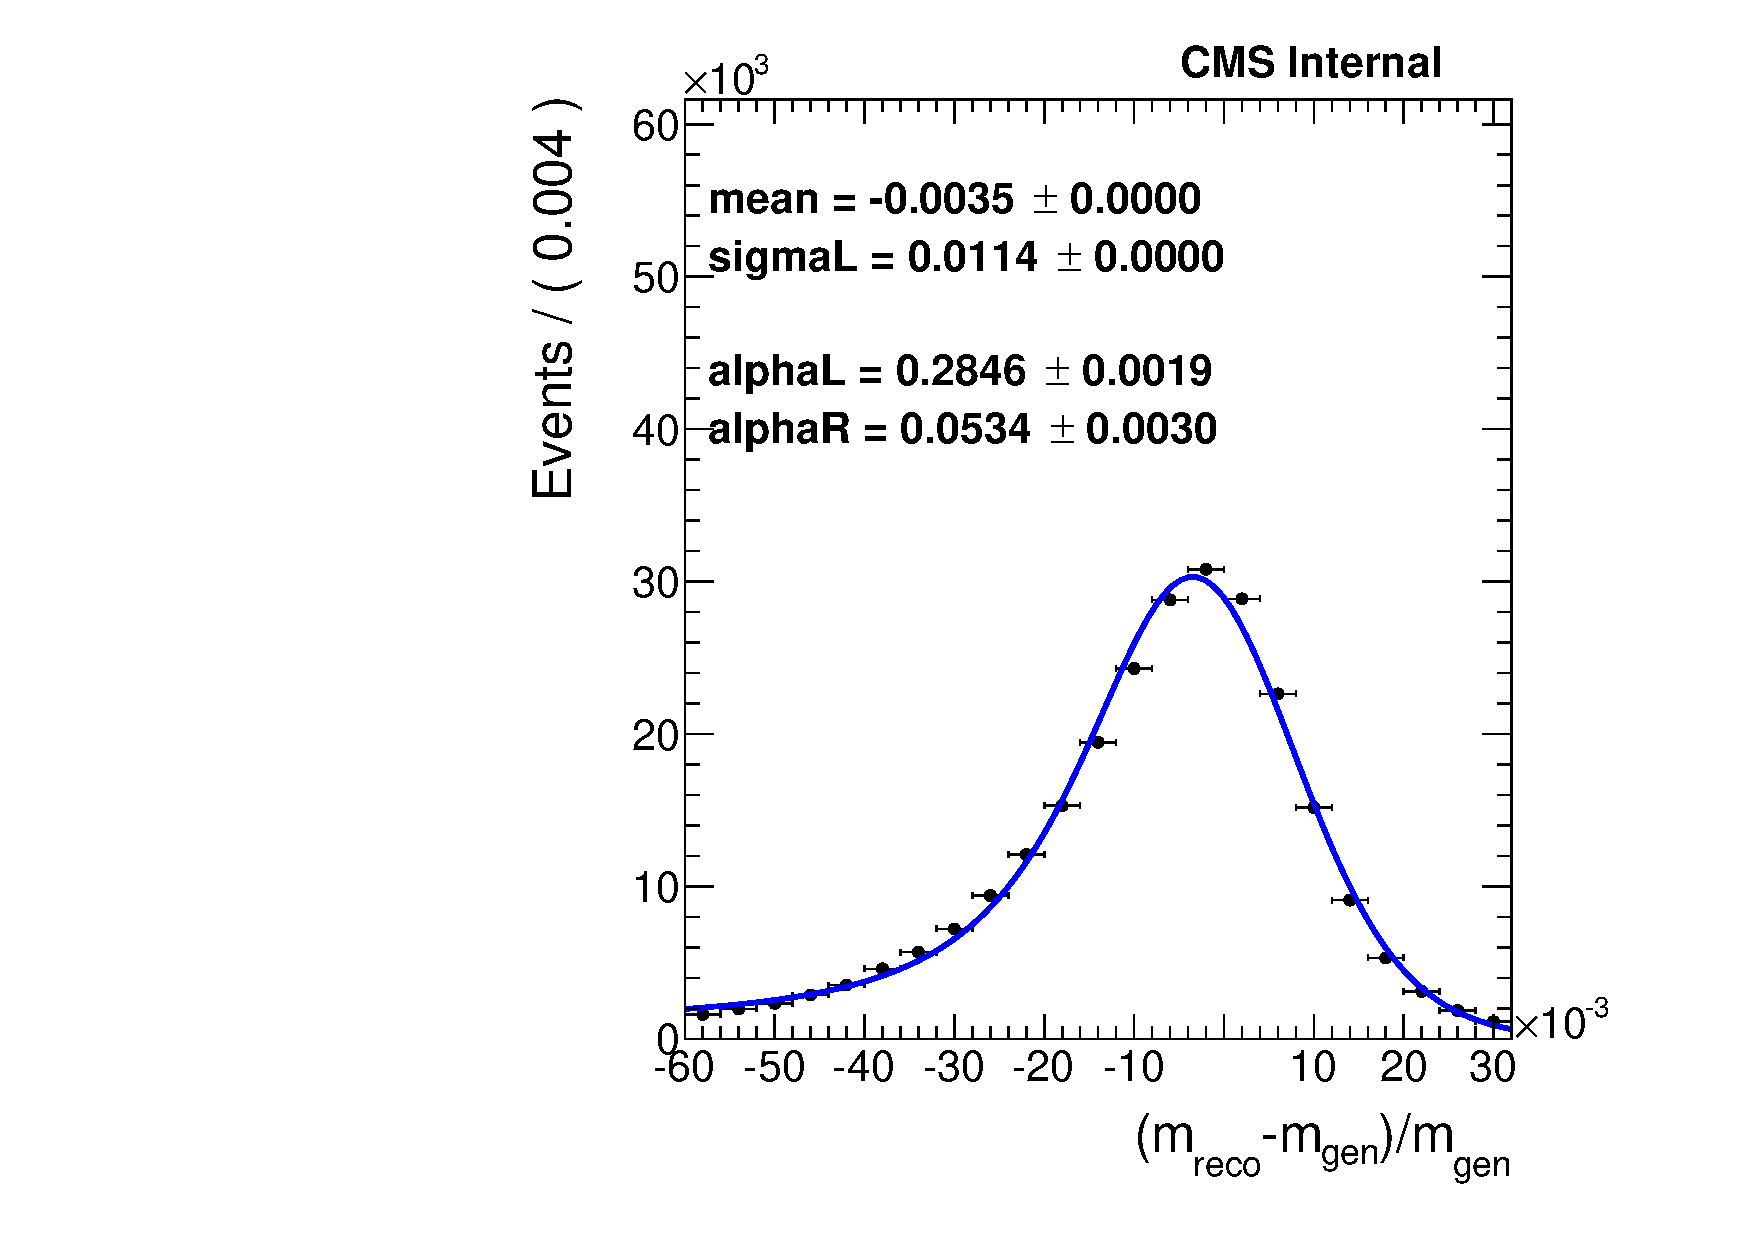
\includegraphics[width=0.22\textwidth]{fig/mass_resolution/Test_fit_results/resolution_BB/h_resolution_BB_1.pdf} &
%      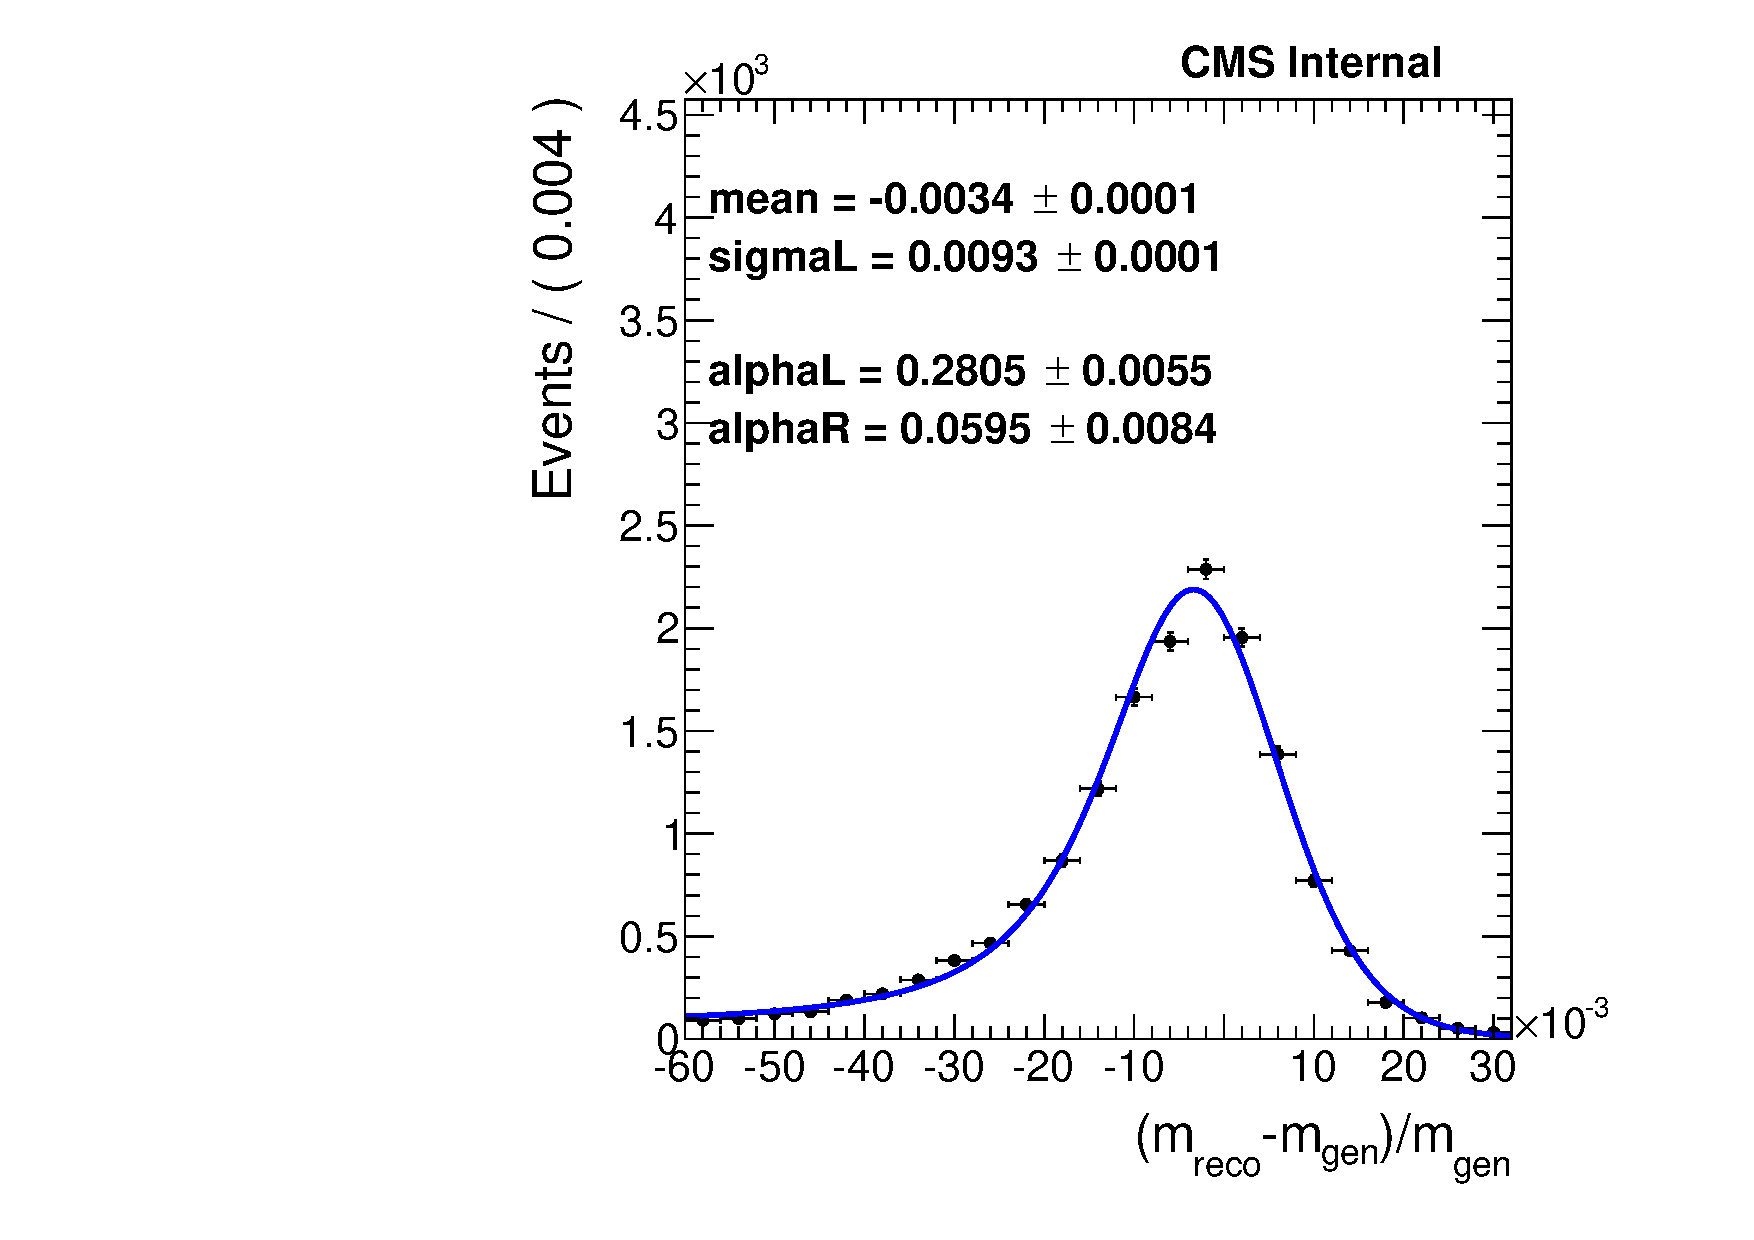
\includegraphics[width=0.22\textwidth]{fig/mass_resolution/Test_fit_results/resolution_BB/h_resolution_BB_2.pdf}&
%      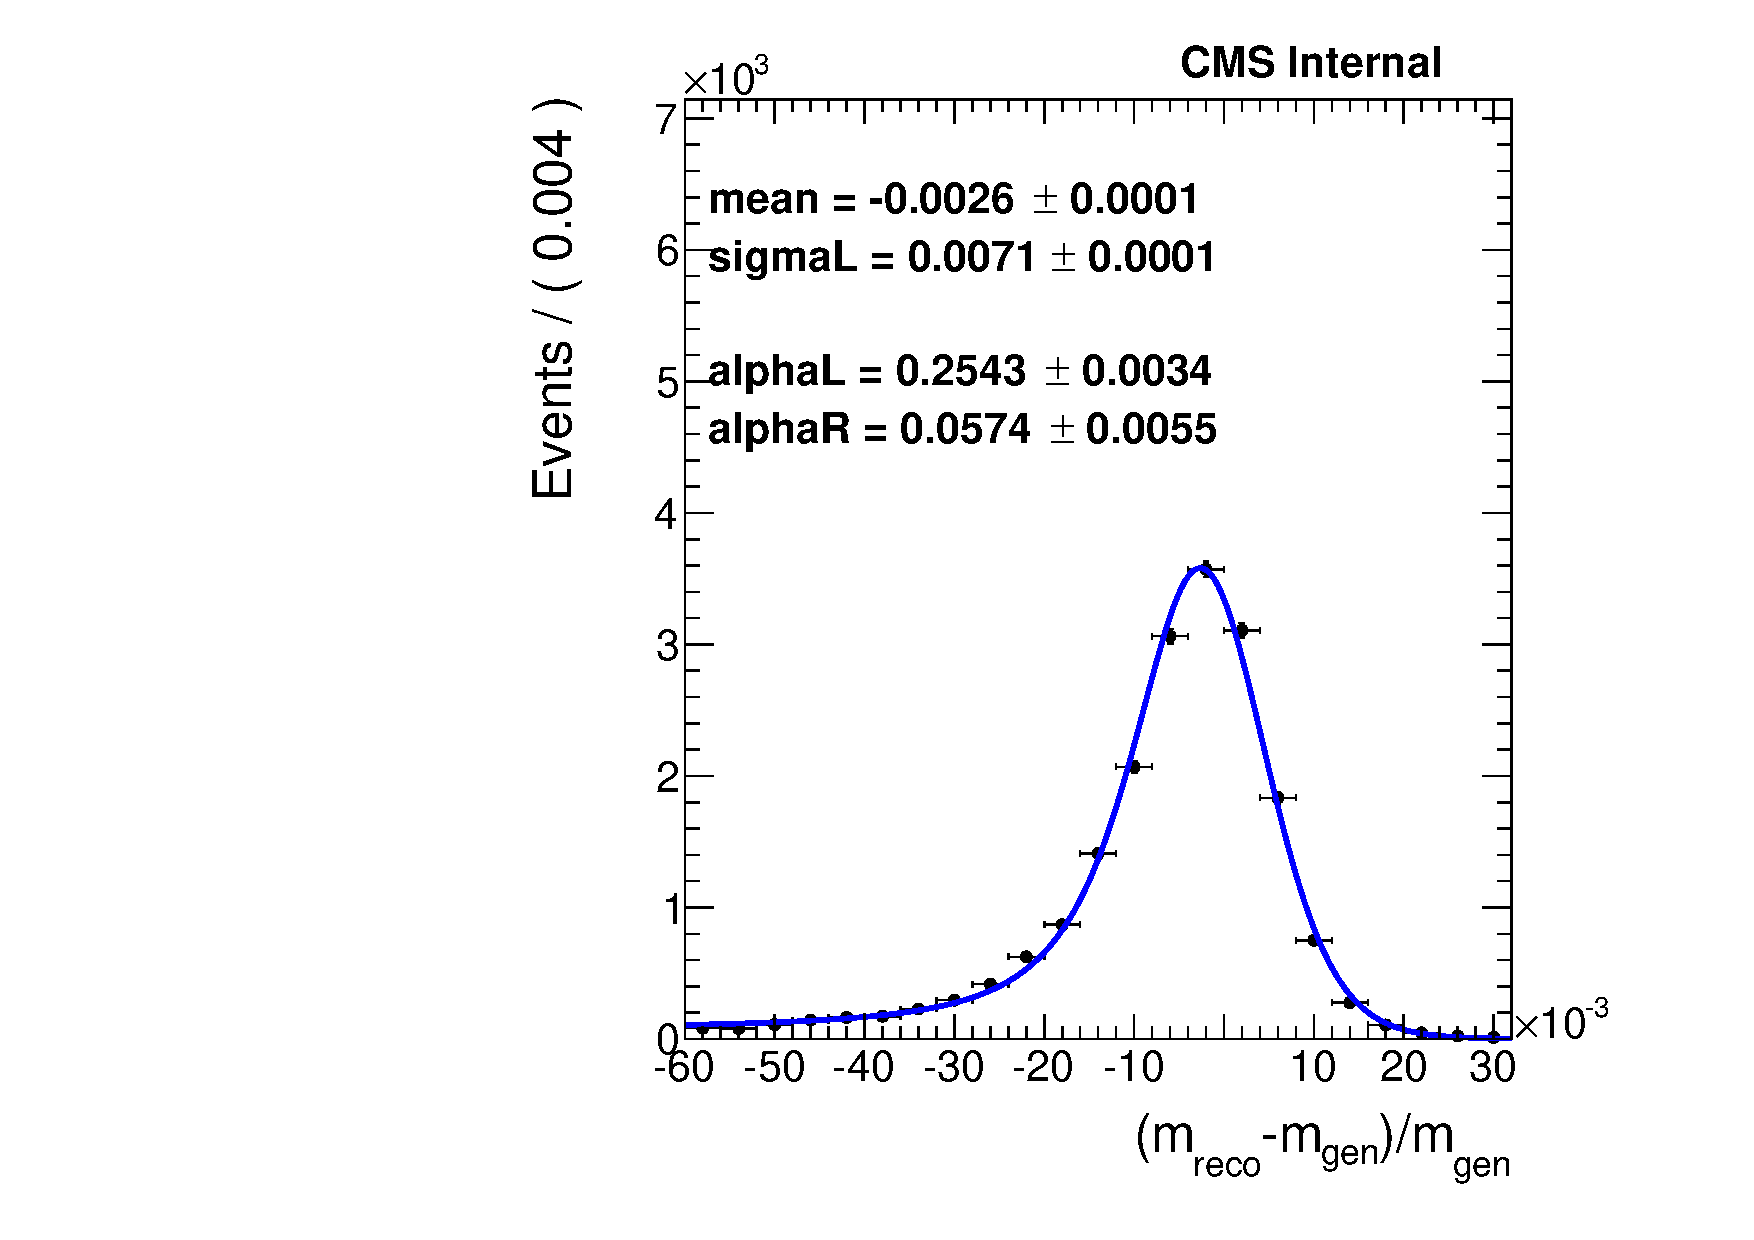
\includegraphics[width=0.22\textwidth]{fig/mass_resolution/Test_fit_results/resolution_BB/h_resolution_BB_3.pdf} &
%      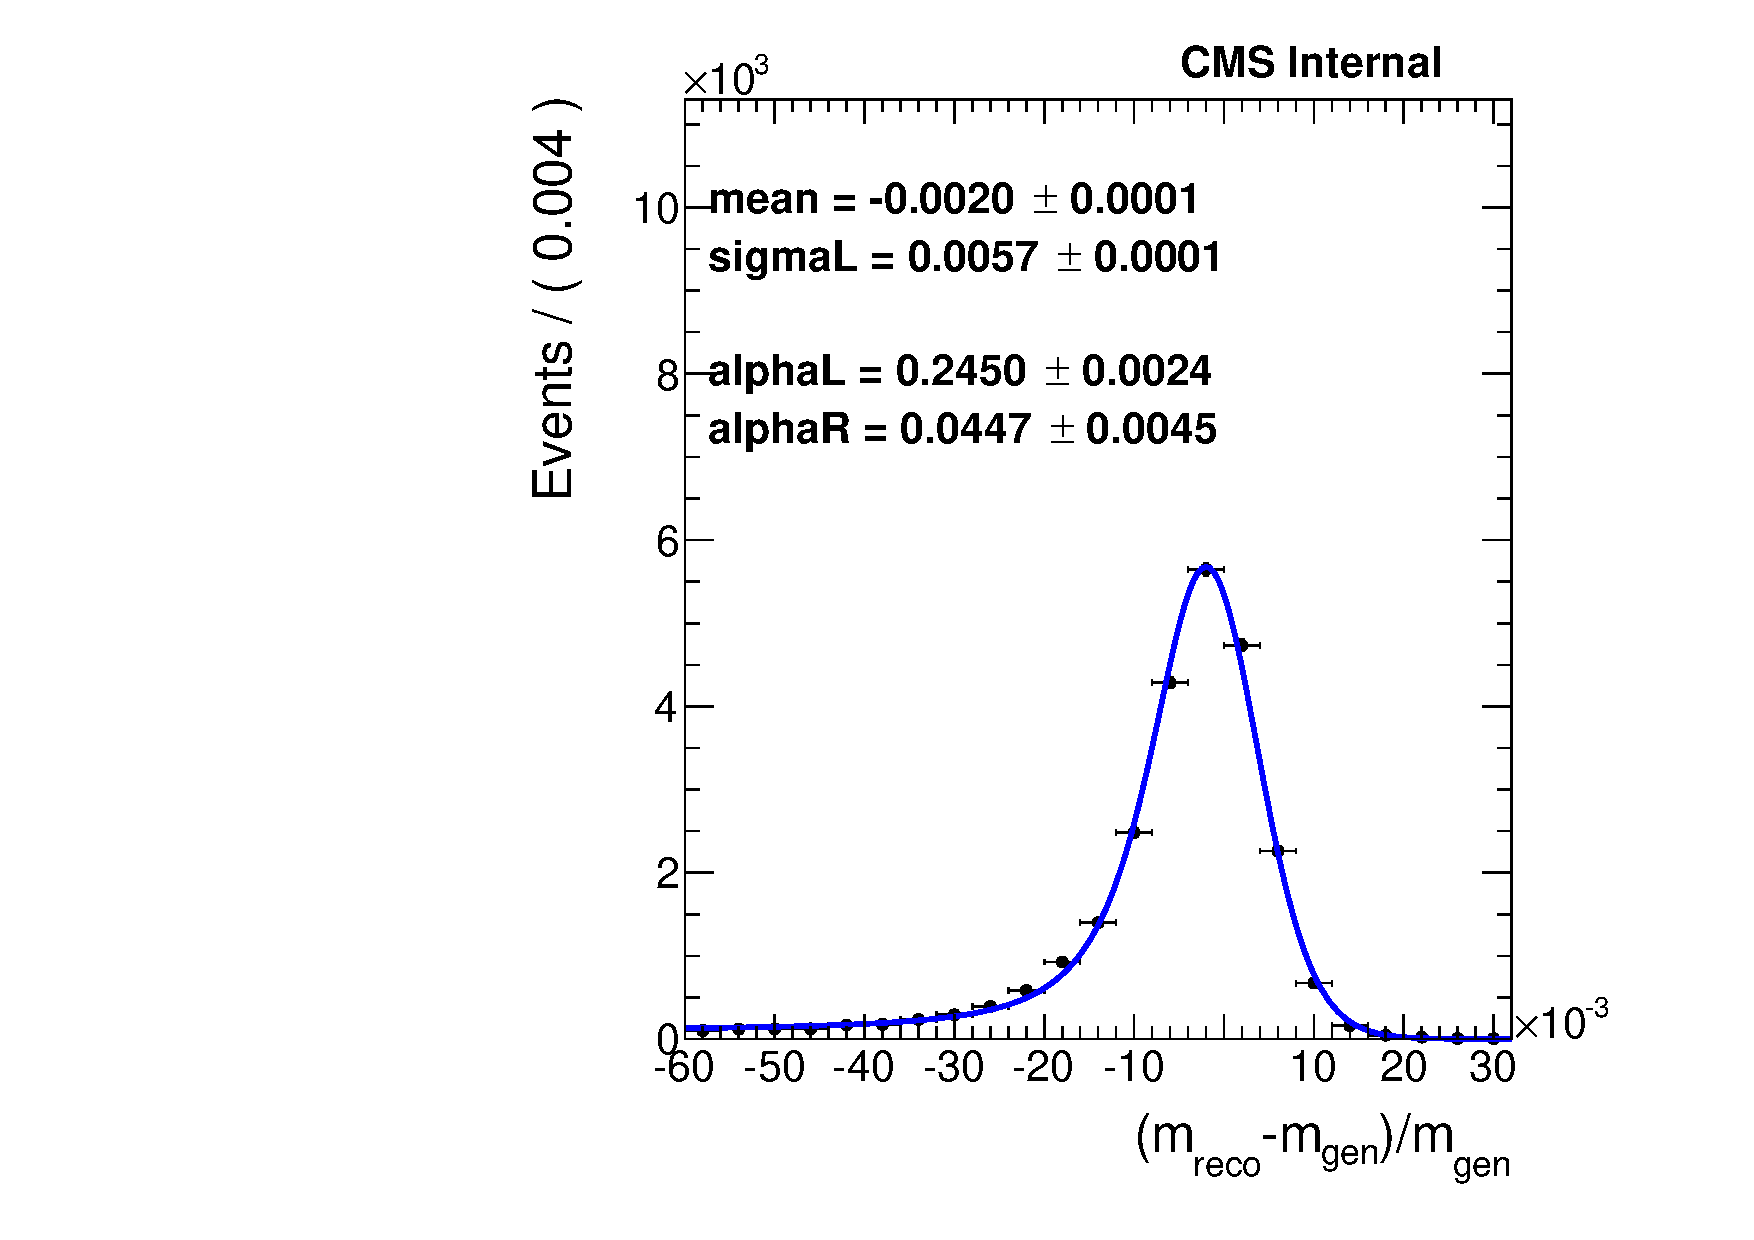
\includegraphics[width=0.22\textwidth]{fig/mass_resolution/Test_fit_results/resolution_BB/h_resolution_BB_4.pdf} \\
%      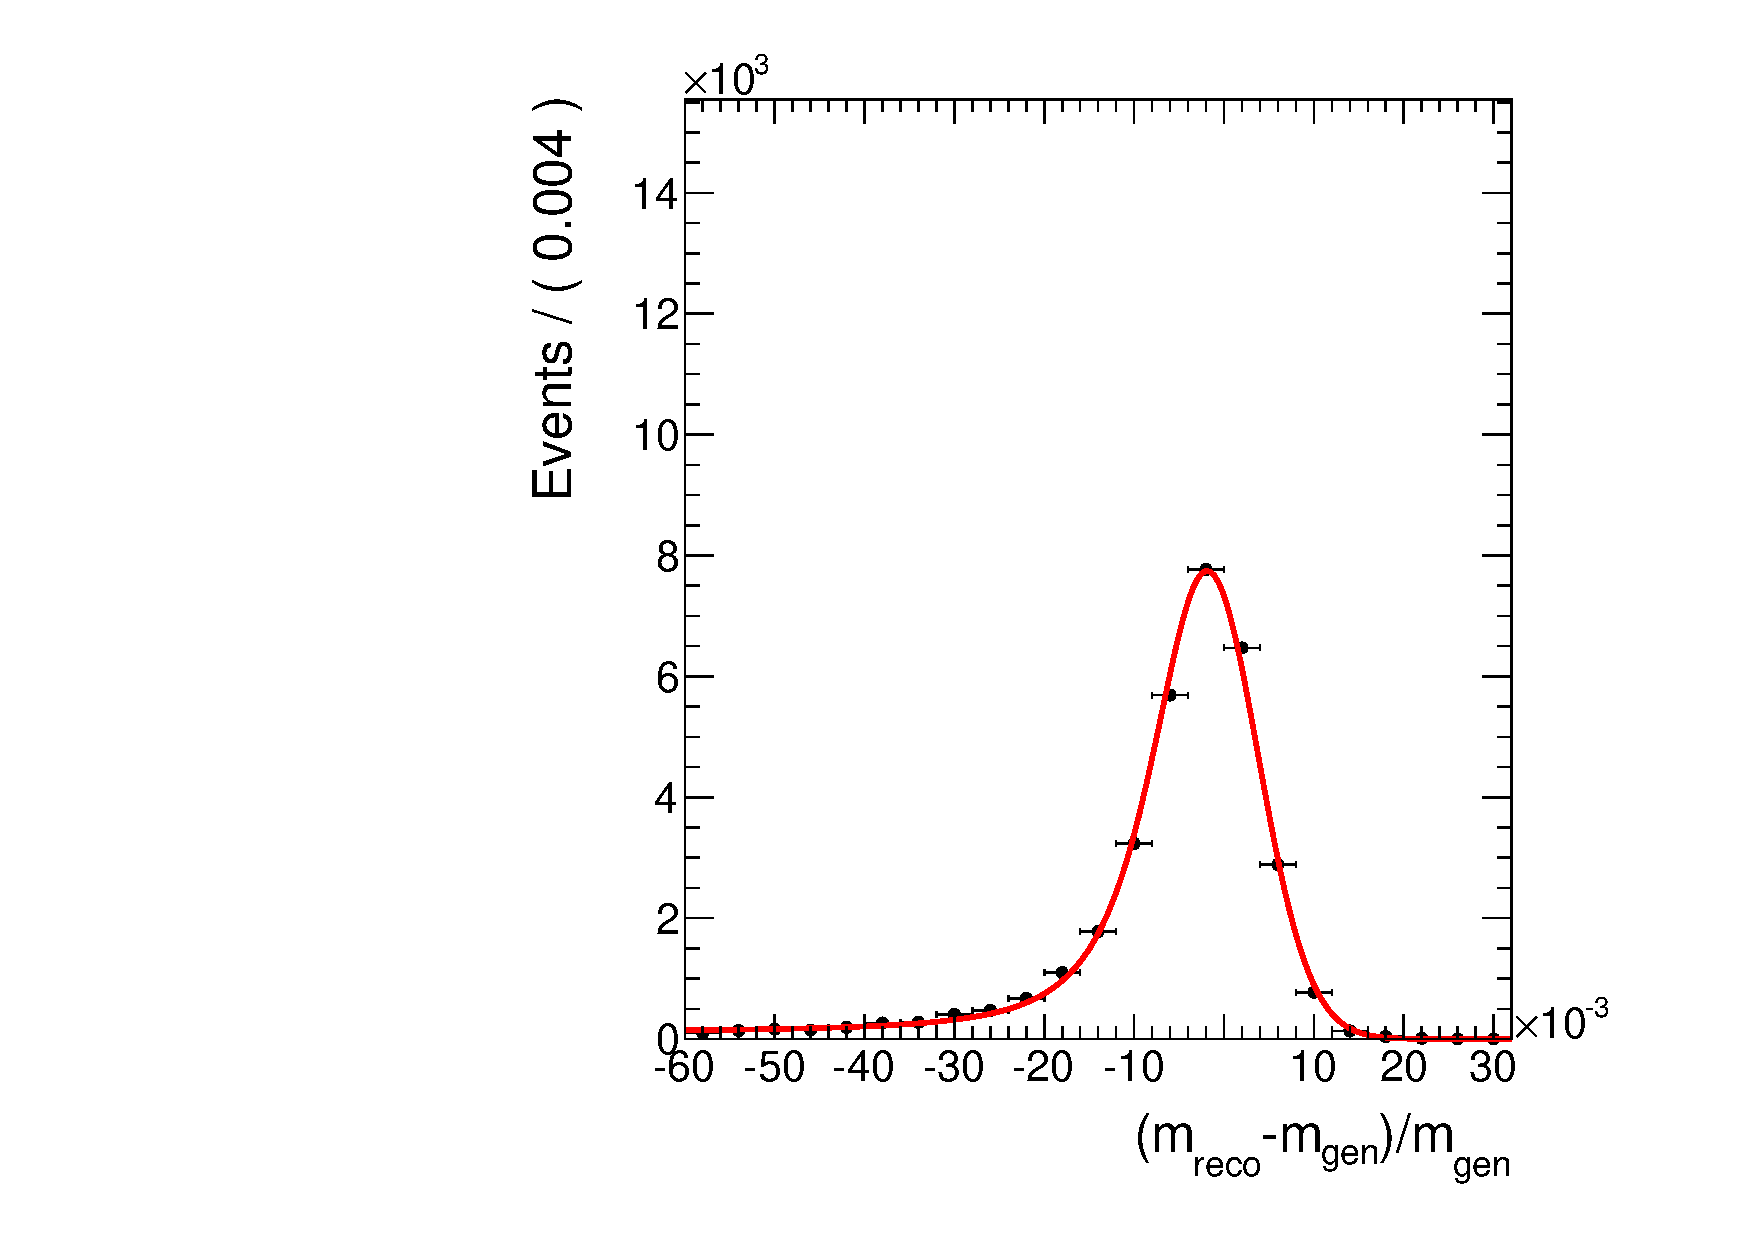
\includegraphics[width=0.22\textwidth]{fig/mass_resolution/Test_fit_results/resolution_BB/h_resolution_BB_5.pdf} &
%      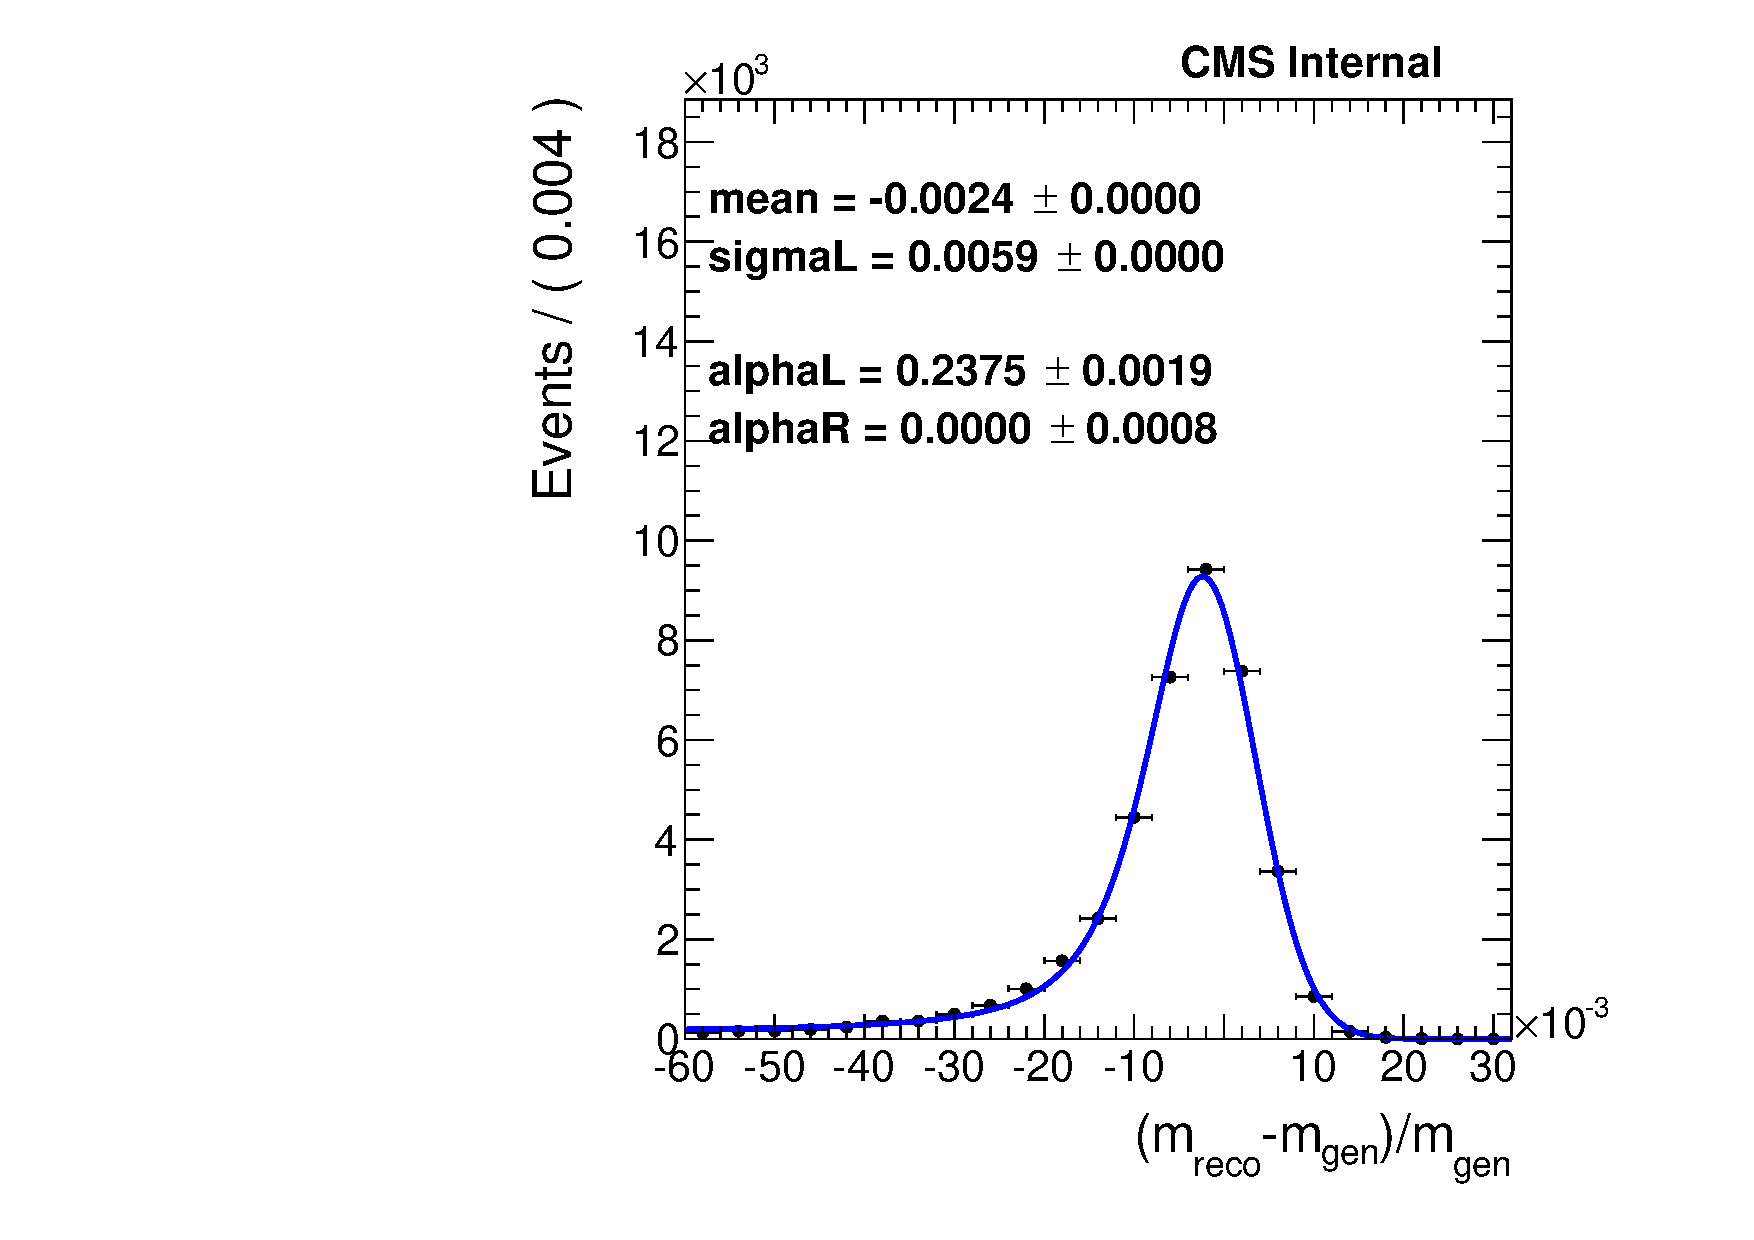
\includegraphics[width=0.22\textwidth]{fig/mass_resolution/Test_fit_results/resolution_BB/h_resolution_BB_6.pdf}&
%      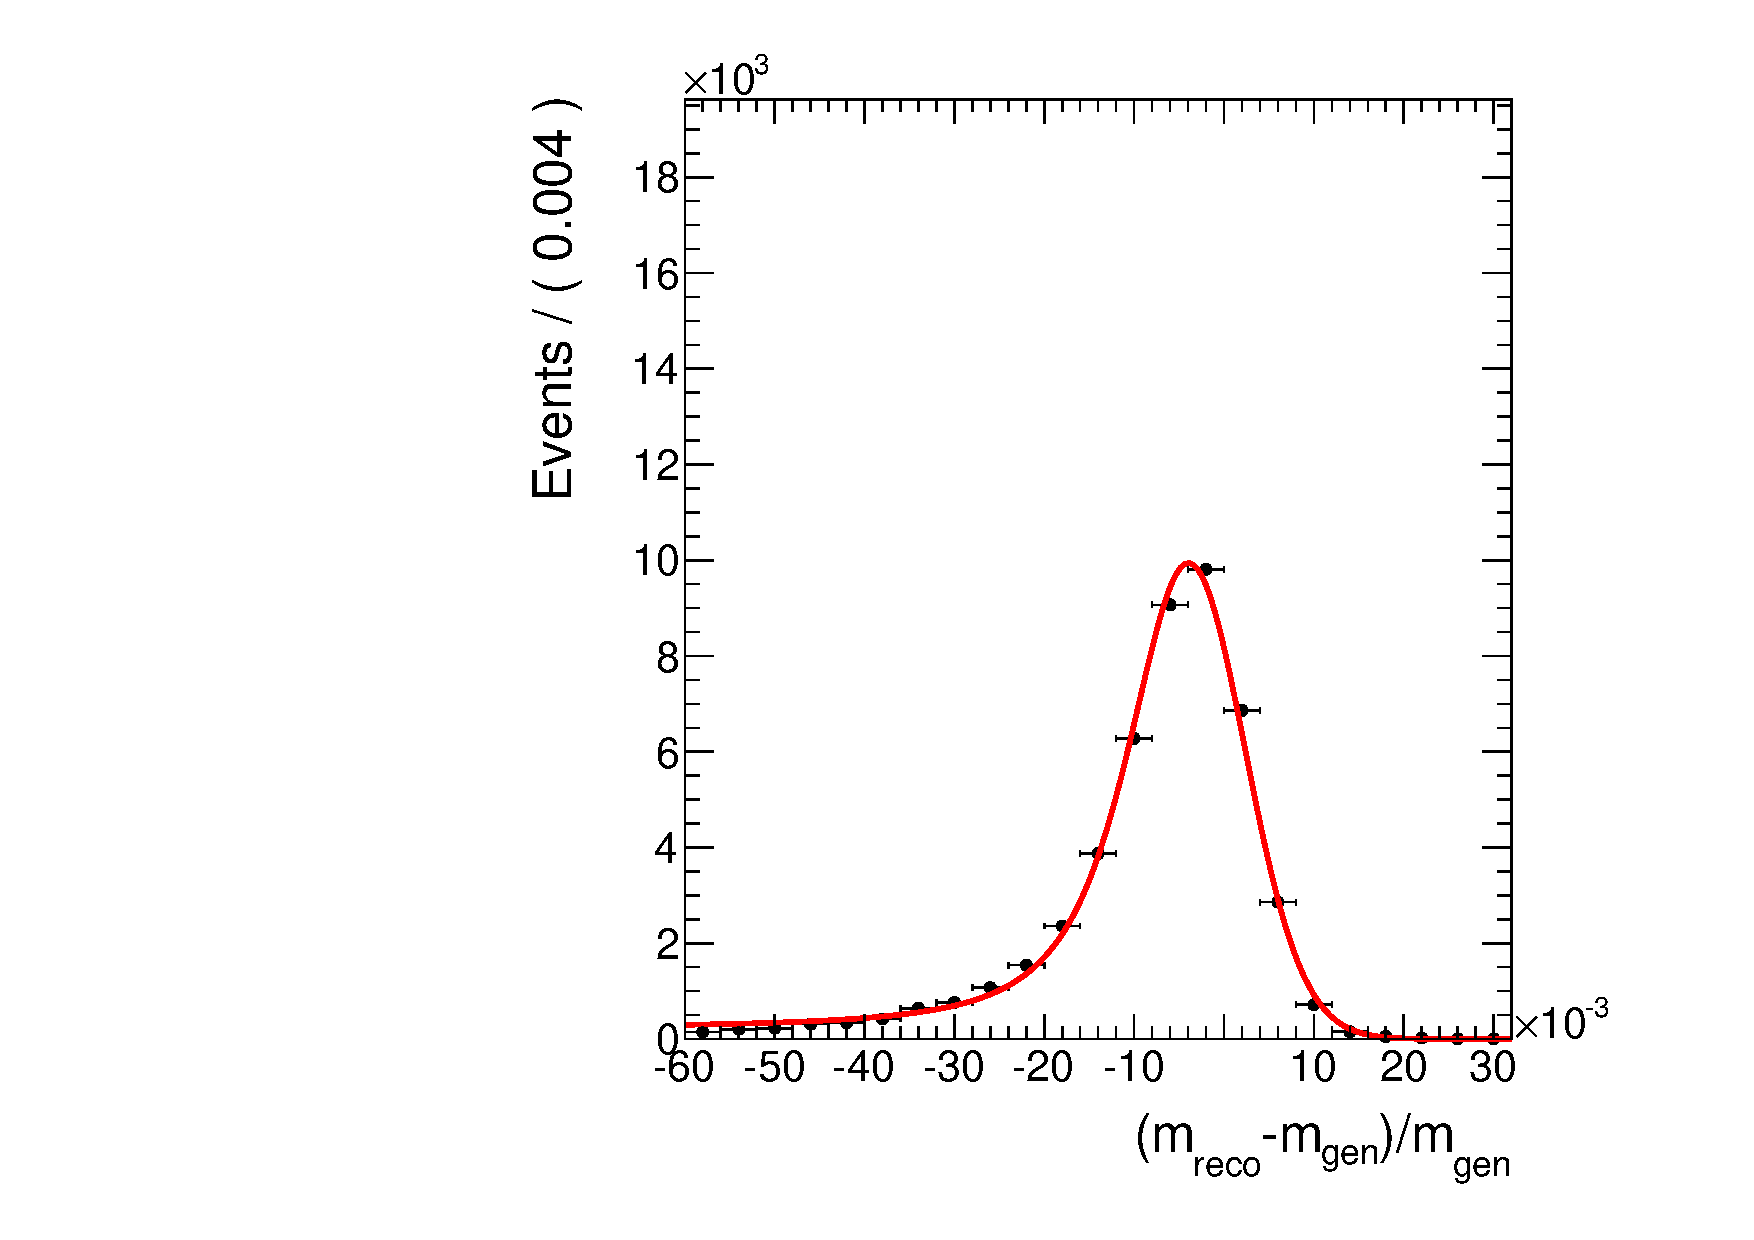
\includegraphics[width=0.22\textwidth]{fig/mass_resolution/Test_fit_results/resolution_BB/h_resolution_BB_7.pdf} &
%      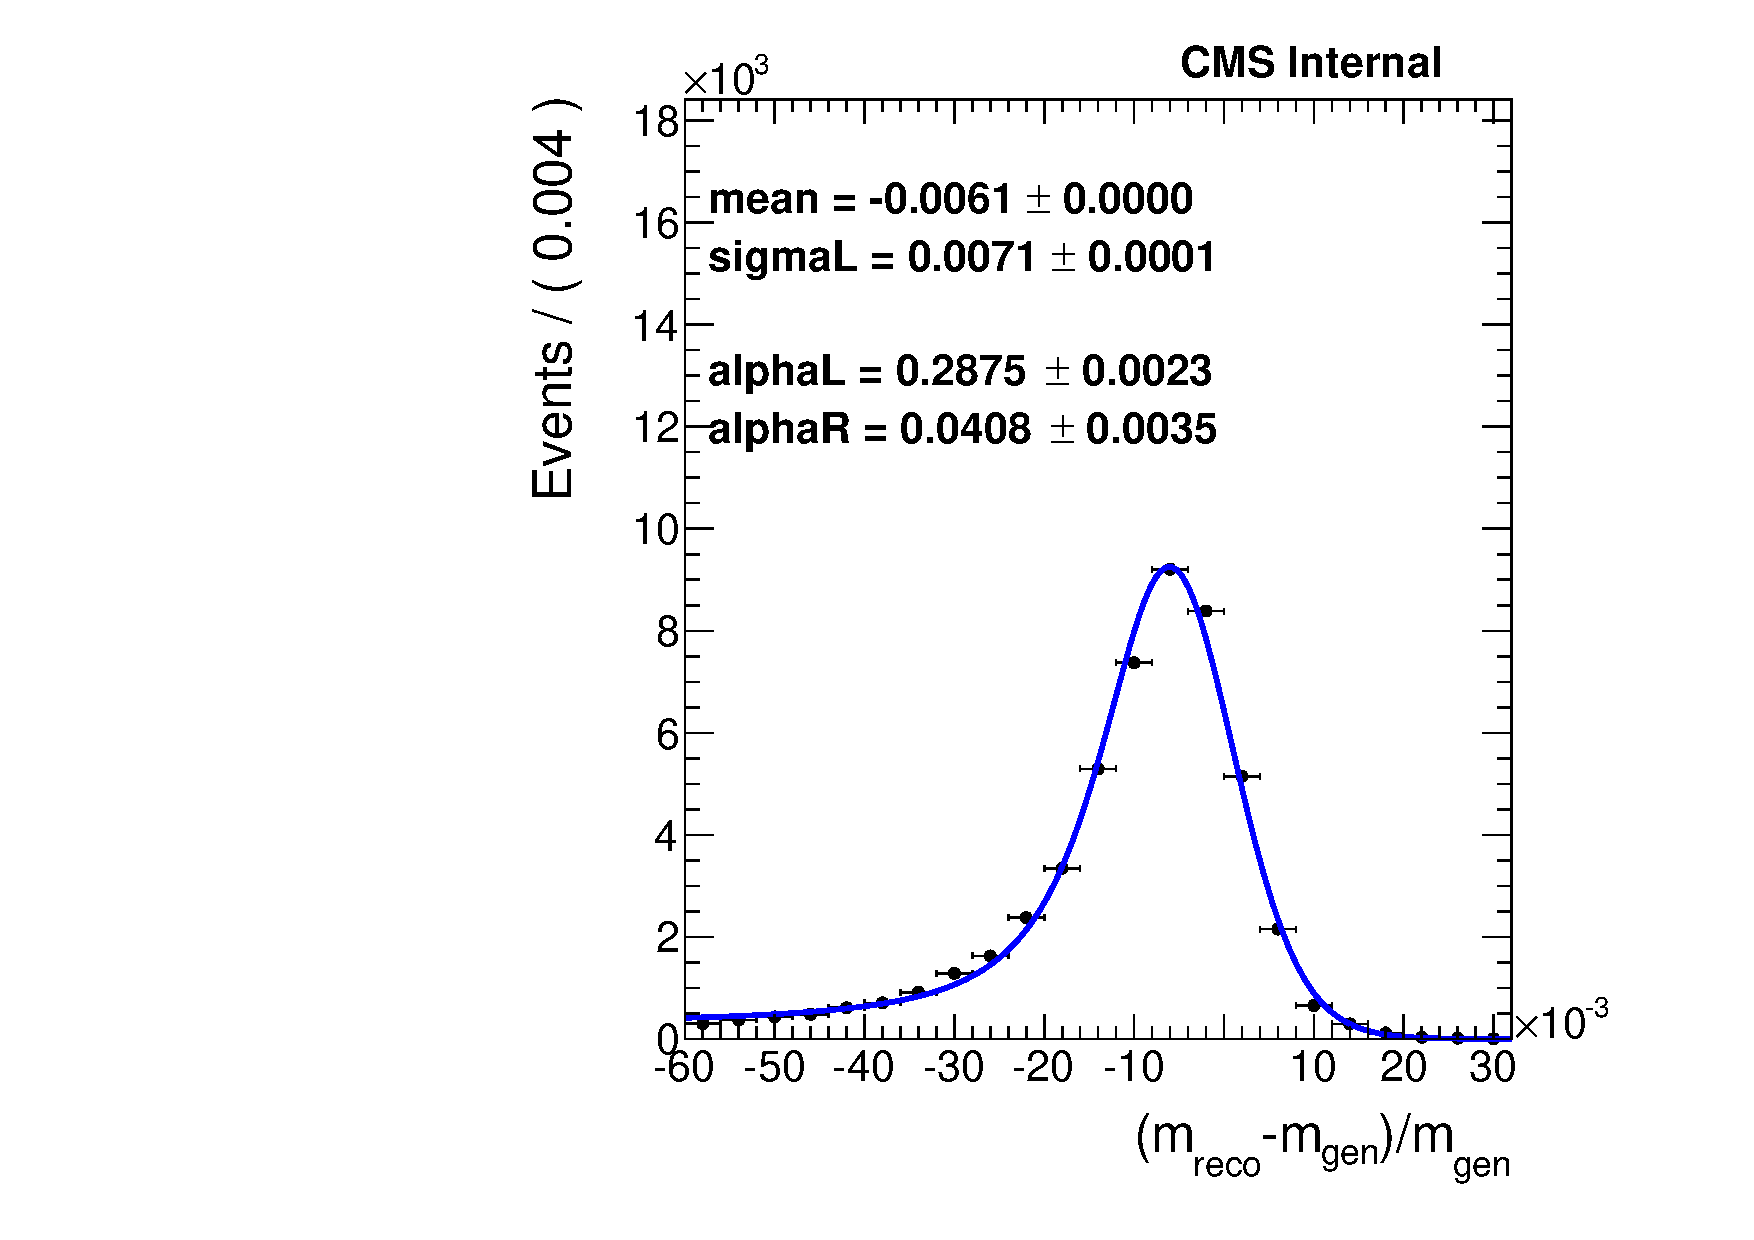
\includegraphics[width=0.22\textwidth]{fig/mass_resolution/Test_fit_results/resolution_BB/h_resolution_BB_8.pdf}\\
%    \end{tabular}
%    \caption{Closure test of the RC description in the BB category.
%    \label{fig:fit_closure_BB}}
%  \end{center}
%\end{figure}
%
%\begin{figure}[ht]
%  \begin{center}
%    \begin{tabular}{cccc}
%      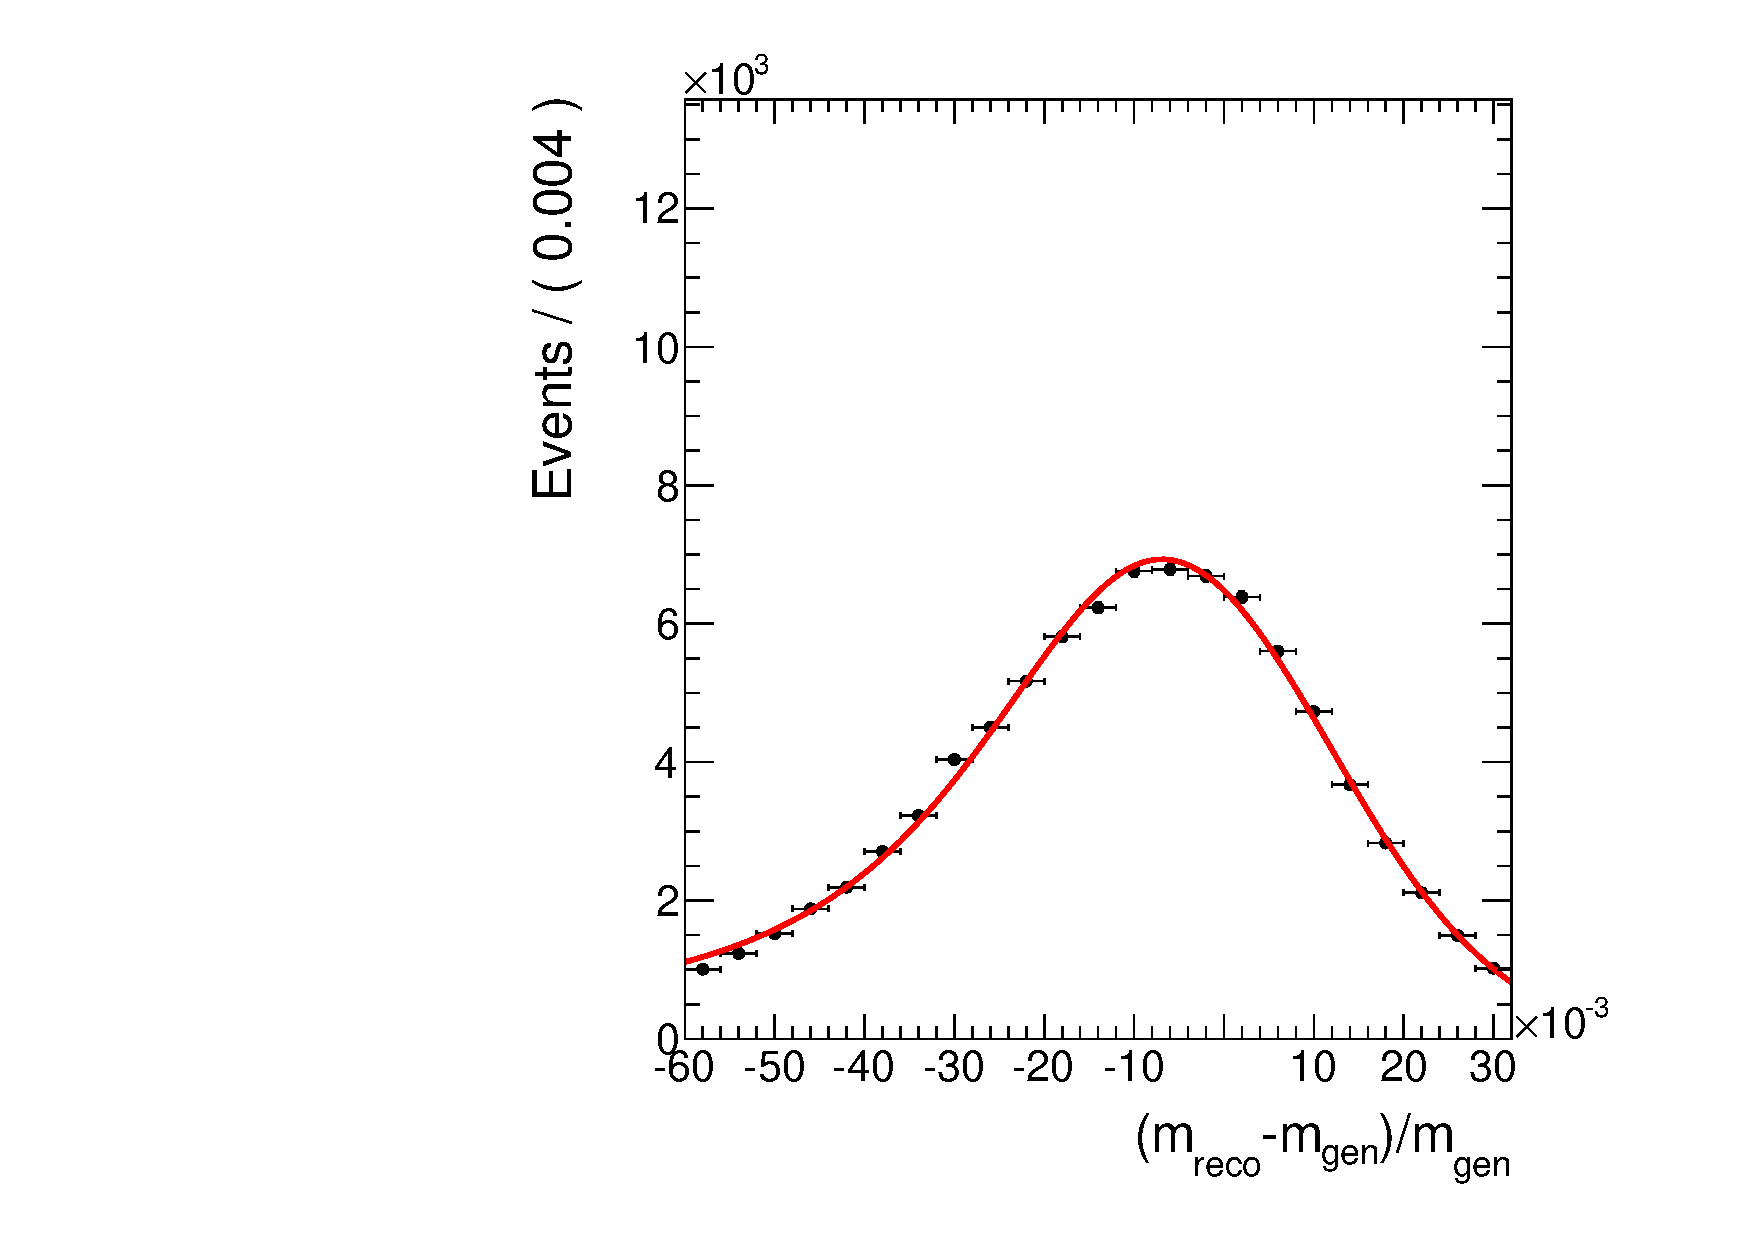
\includegraphics[width=0.22\textwidth]{fig/mass_resolution/Test_fit_results/resolution_BE/h_resolution_BE_1.pdf} &
%      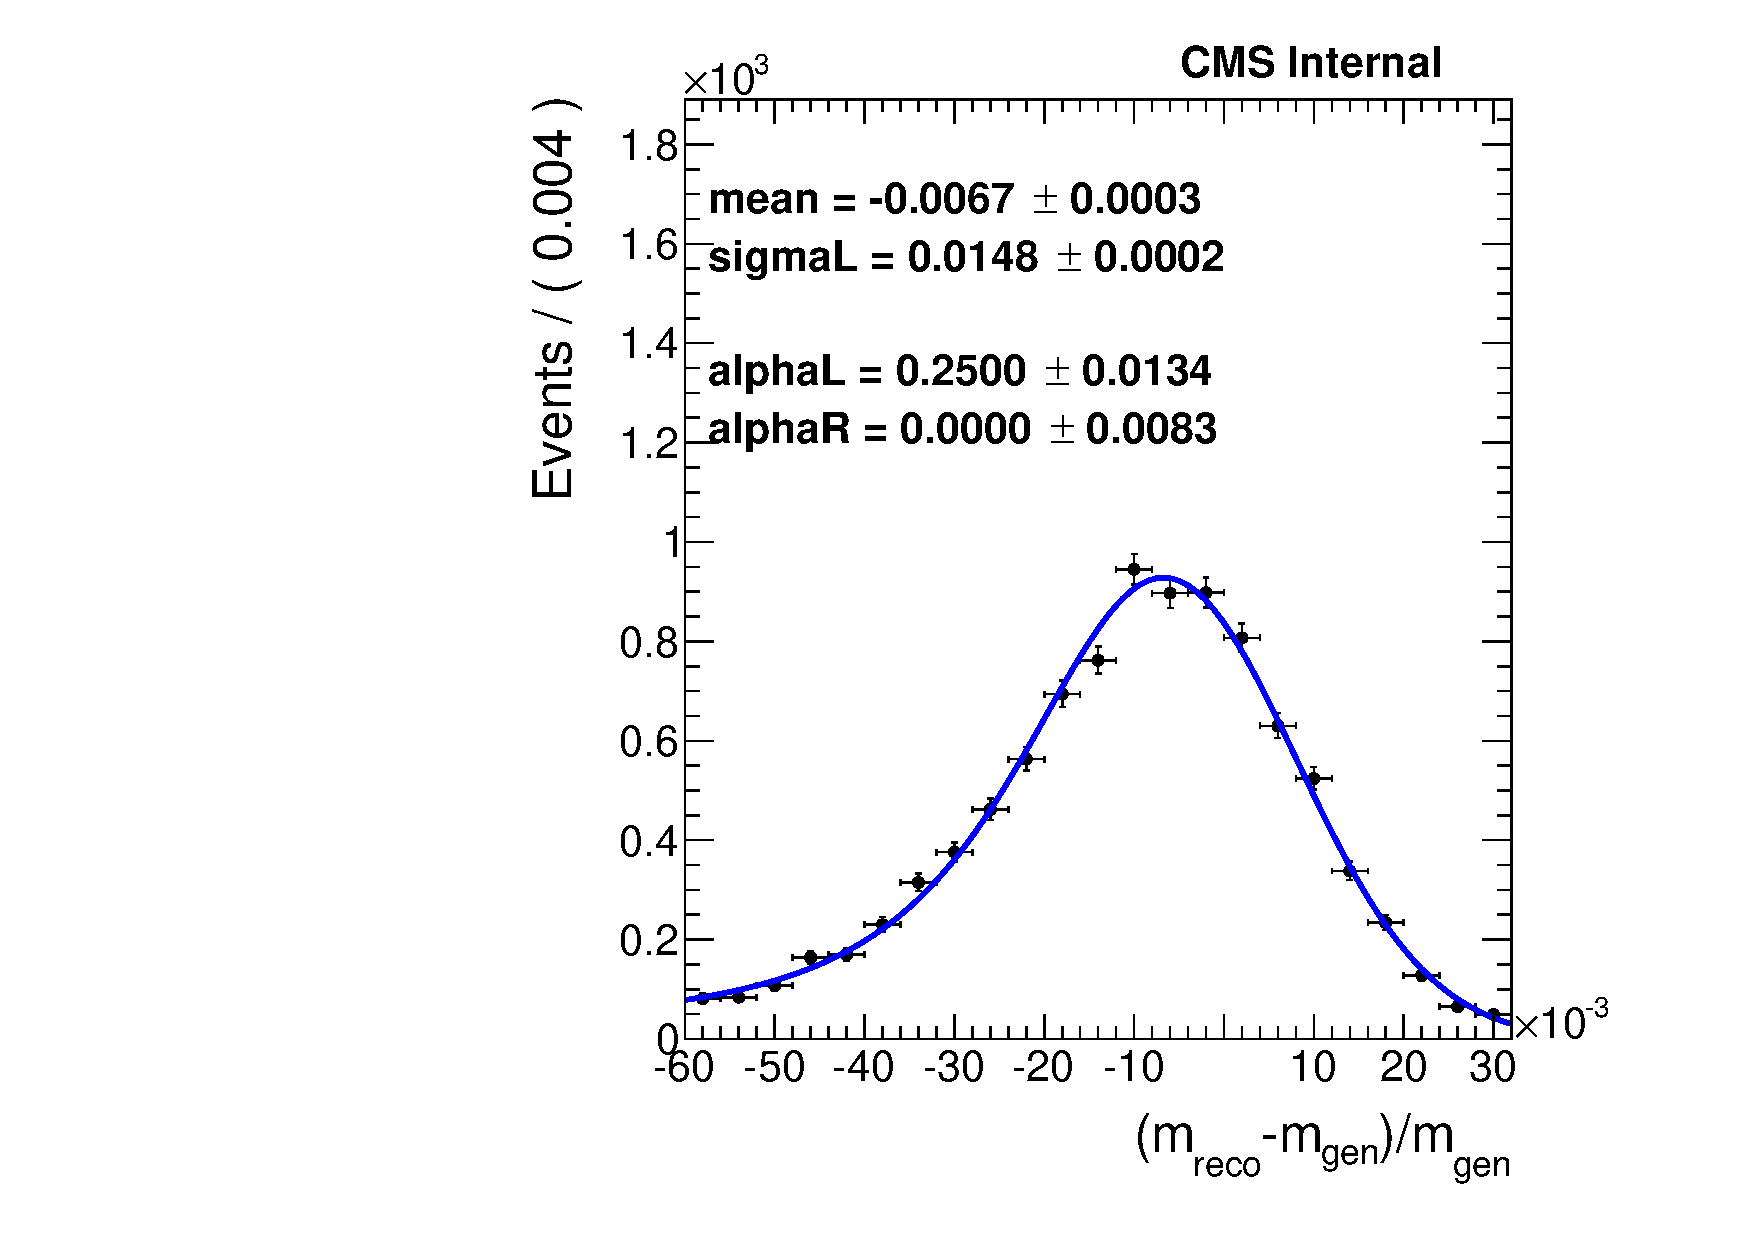
\includegraphics[width=0.22\textwidth]{fig/mass_resolution/Test_fit_results/resolution_BE/h_resolution_BE_2.pdf}&
%      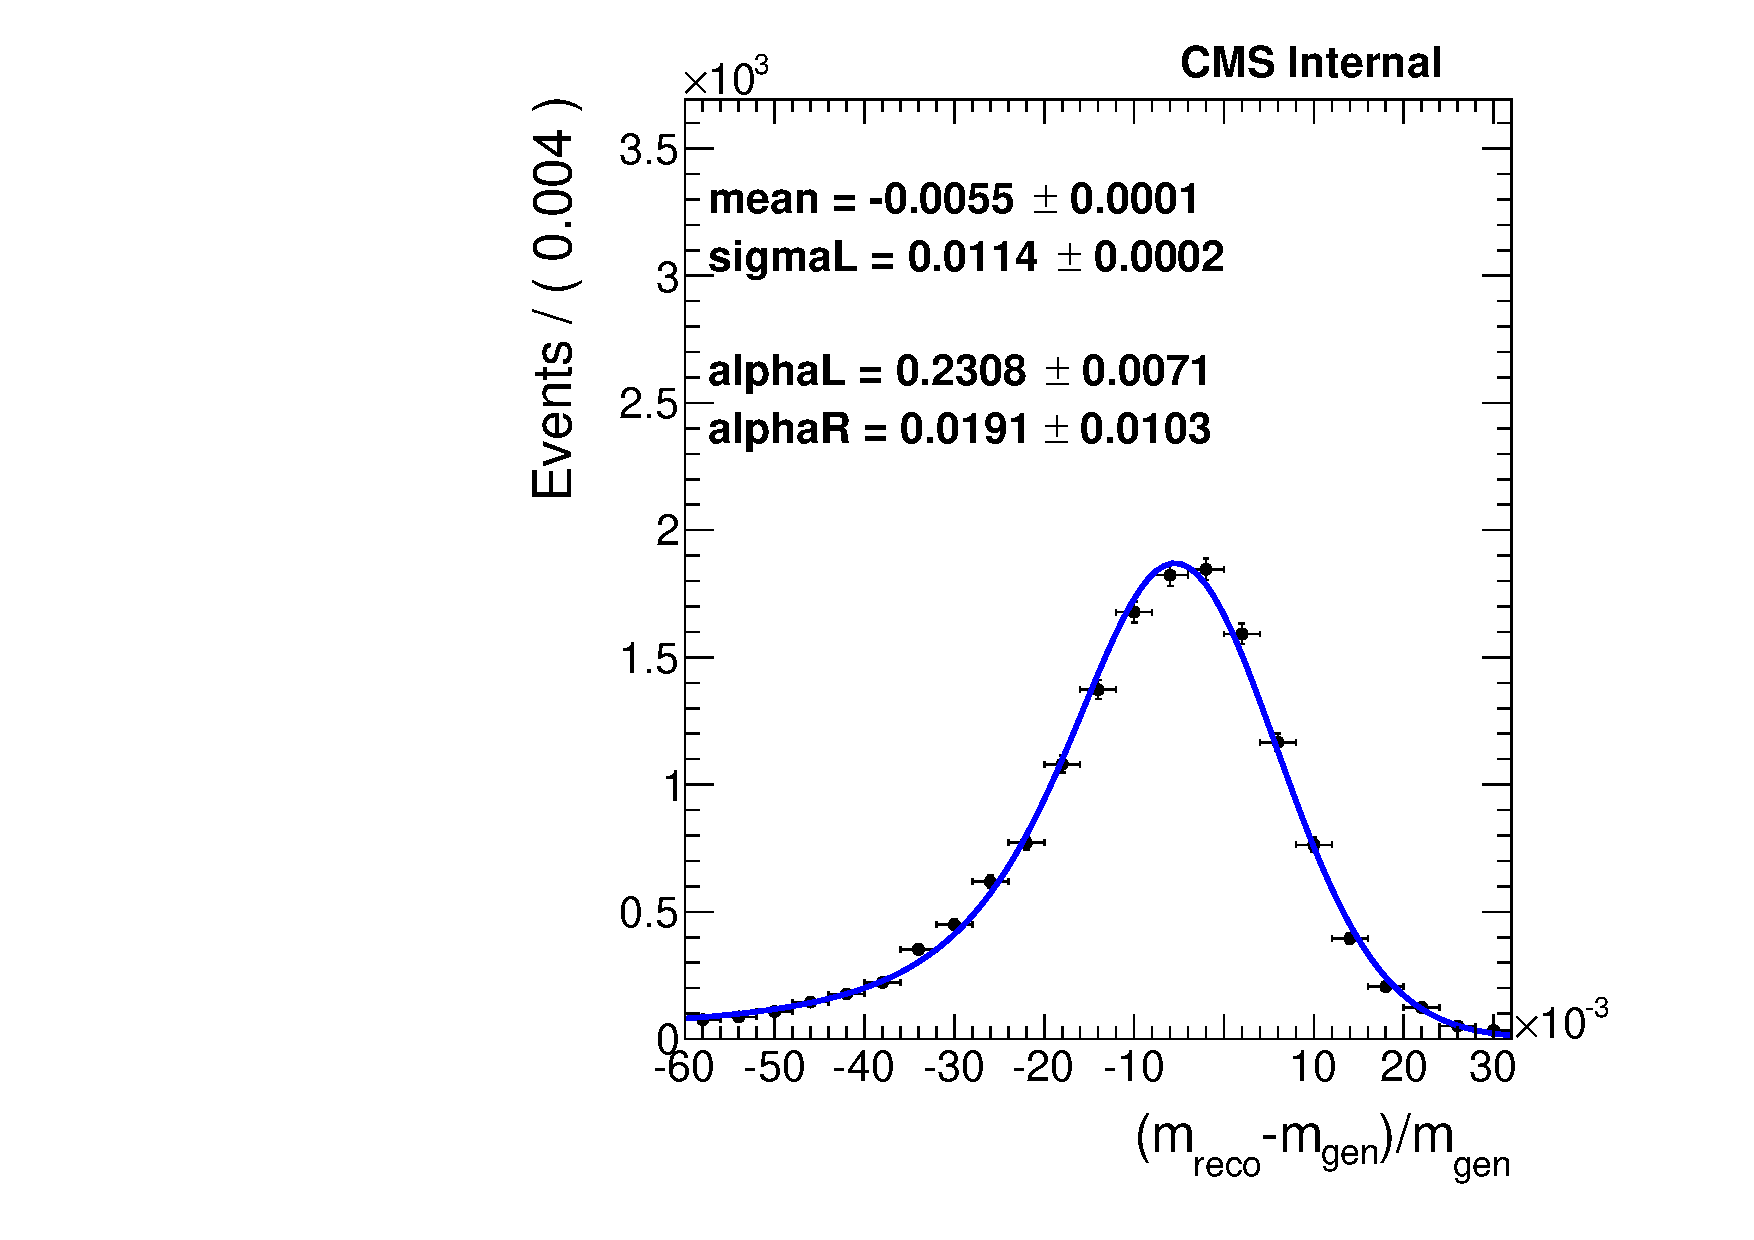
\includegraphics[width=0.22\textwidth]{fig/mass_resolution/Test_fit_results/resolution_BE/h_resolution_BE_3.pdf} &
%      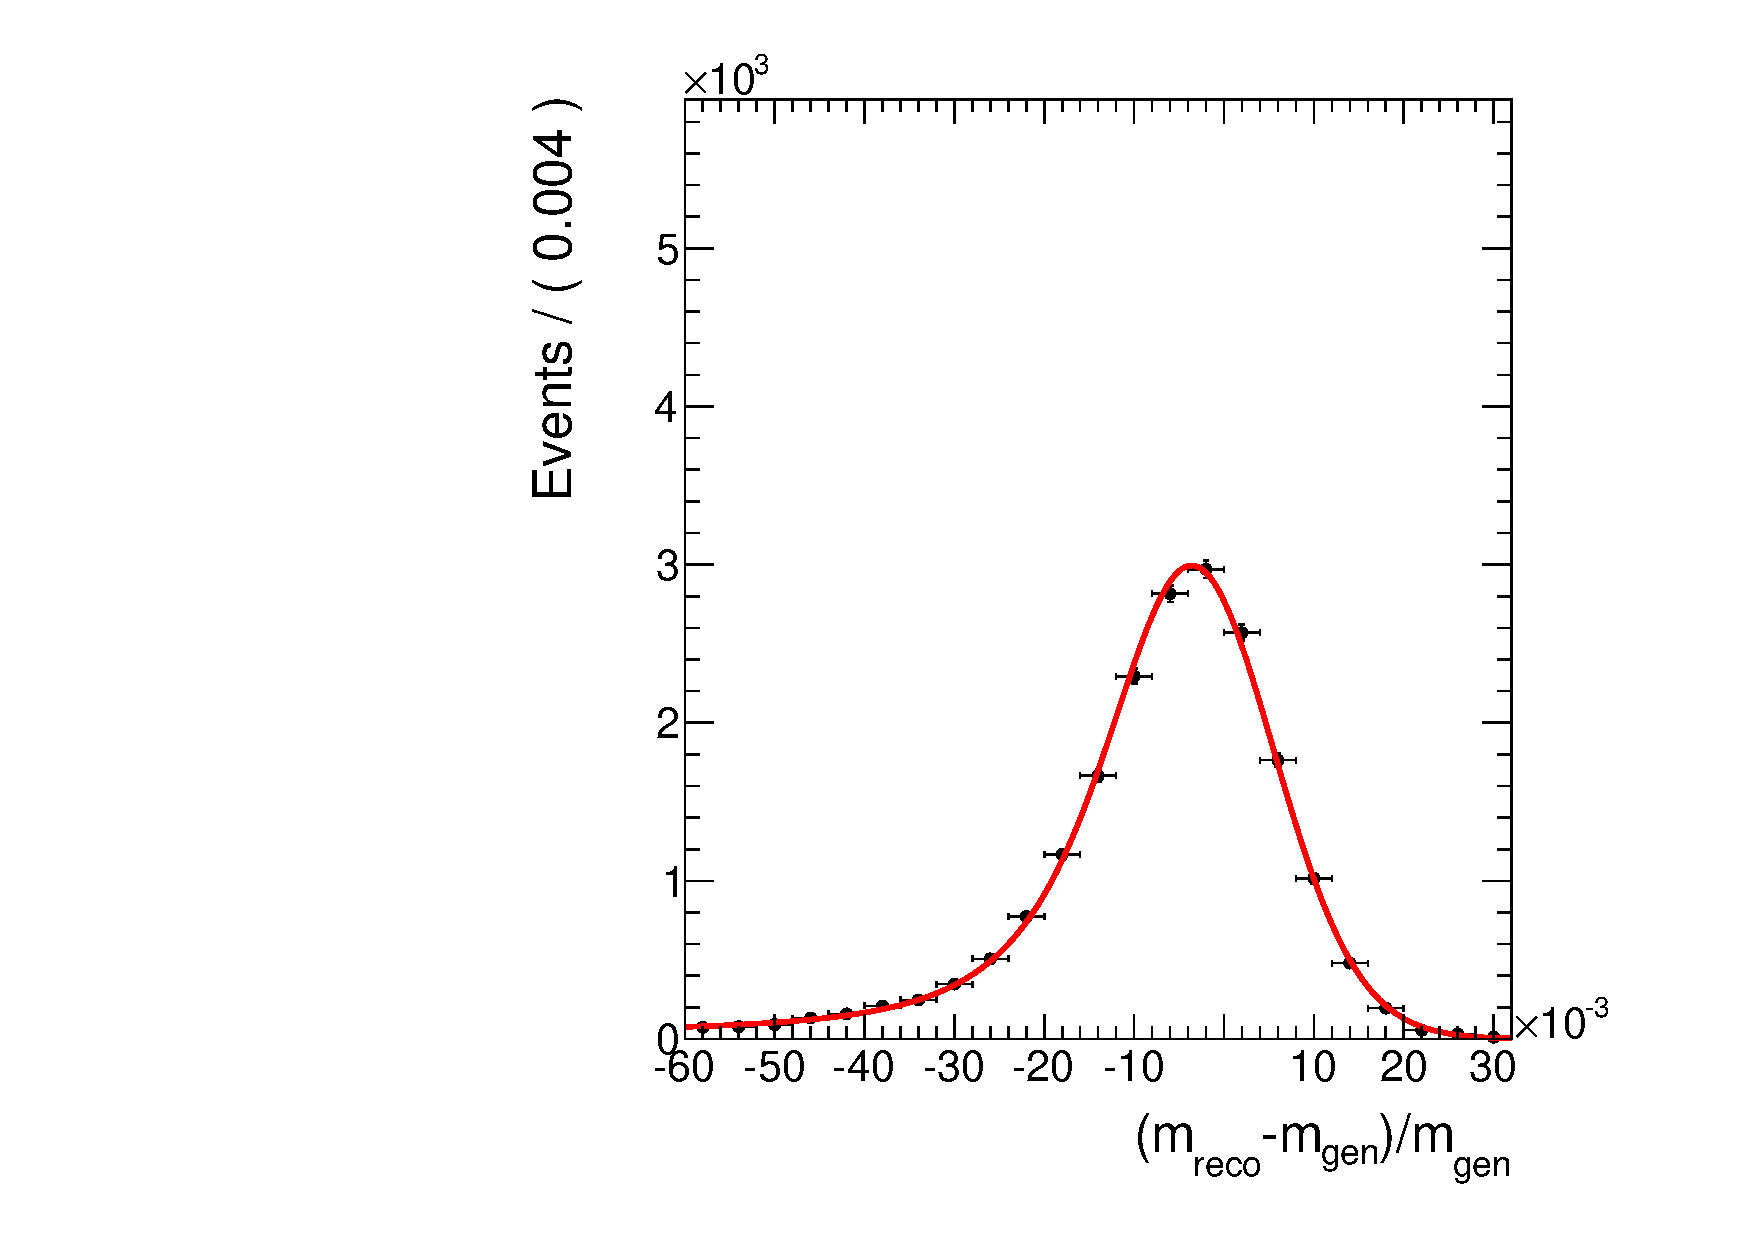
\includegraphics[width=0.22\textwidth]{fig/mass_resolution/Test_fit_results/resolution_BE/h_resolution_BE_4.pdf} \\
%      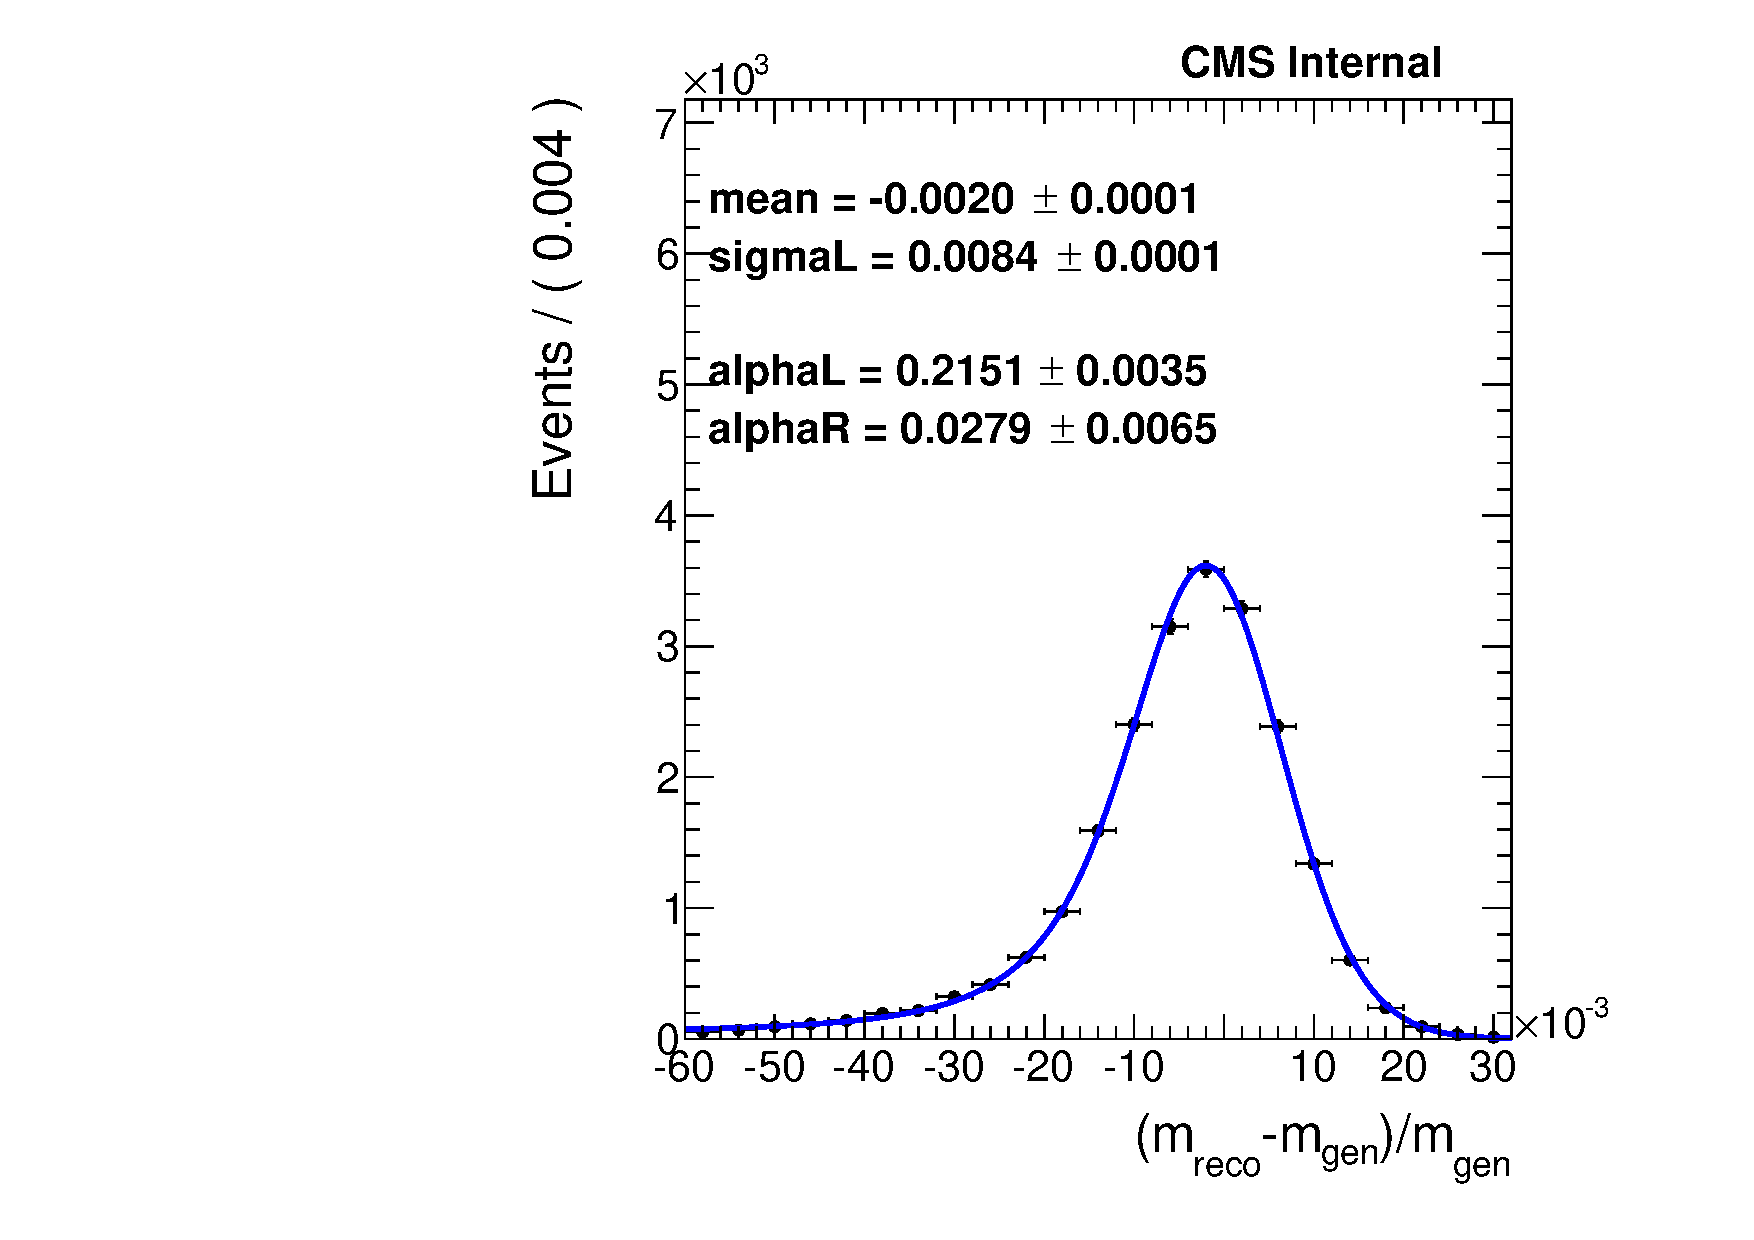
\includegraphics[width=0.22\textwidth]{fig/mass_resolution/Test_fit_results/resolution_BE/h_resolution_BE_5.pdf} &
%      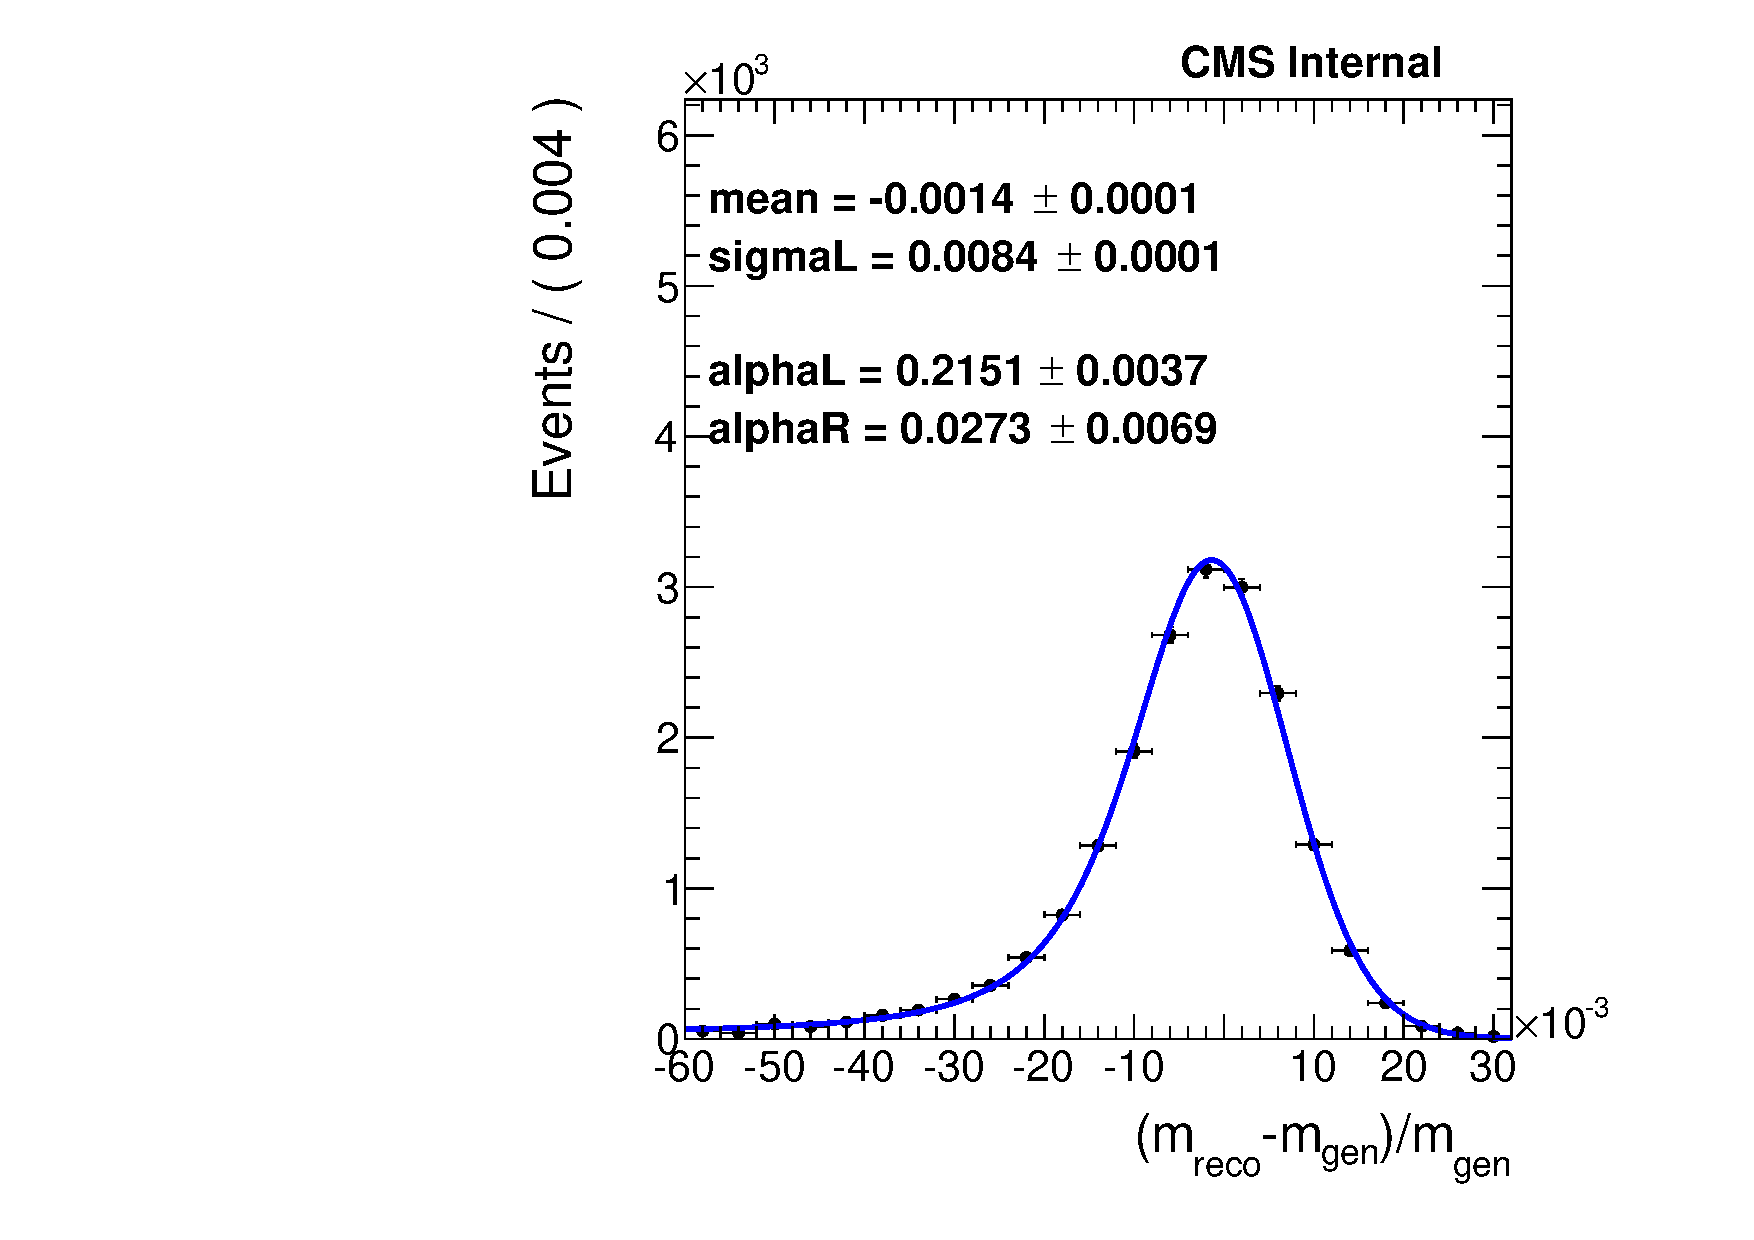
\includegraphics[width=0.22\textwidth]{fig/mass_resolution/Test_fit_results/resolution_BE/h_resolution_BE_6.pdf}&
%      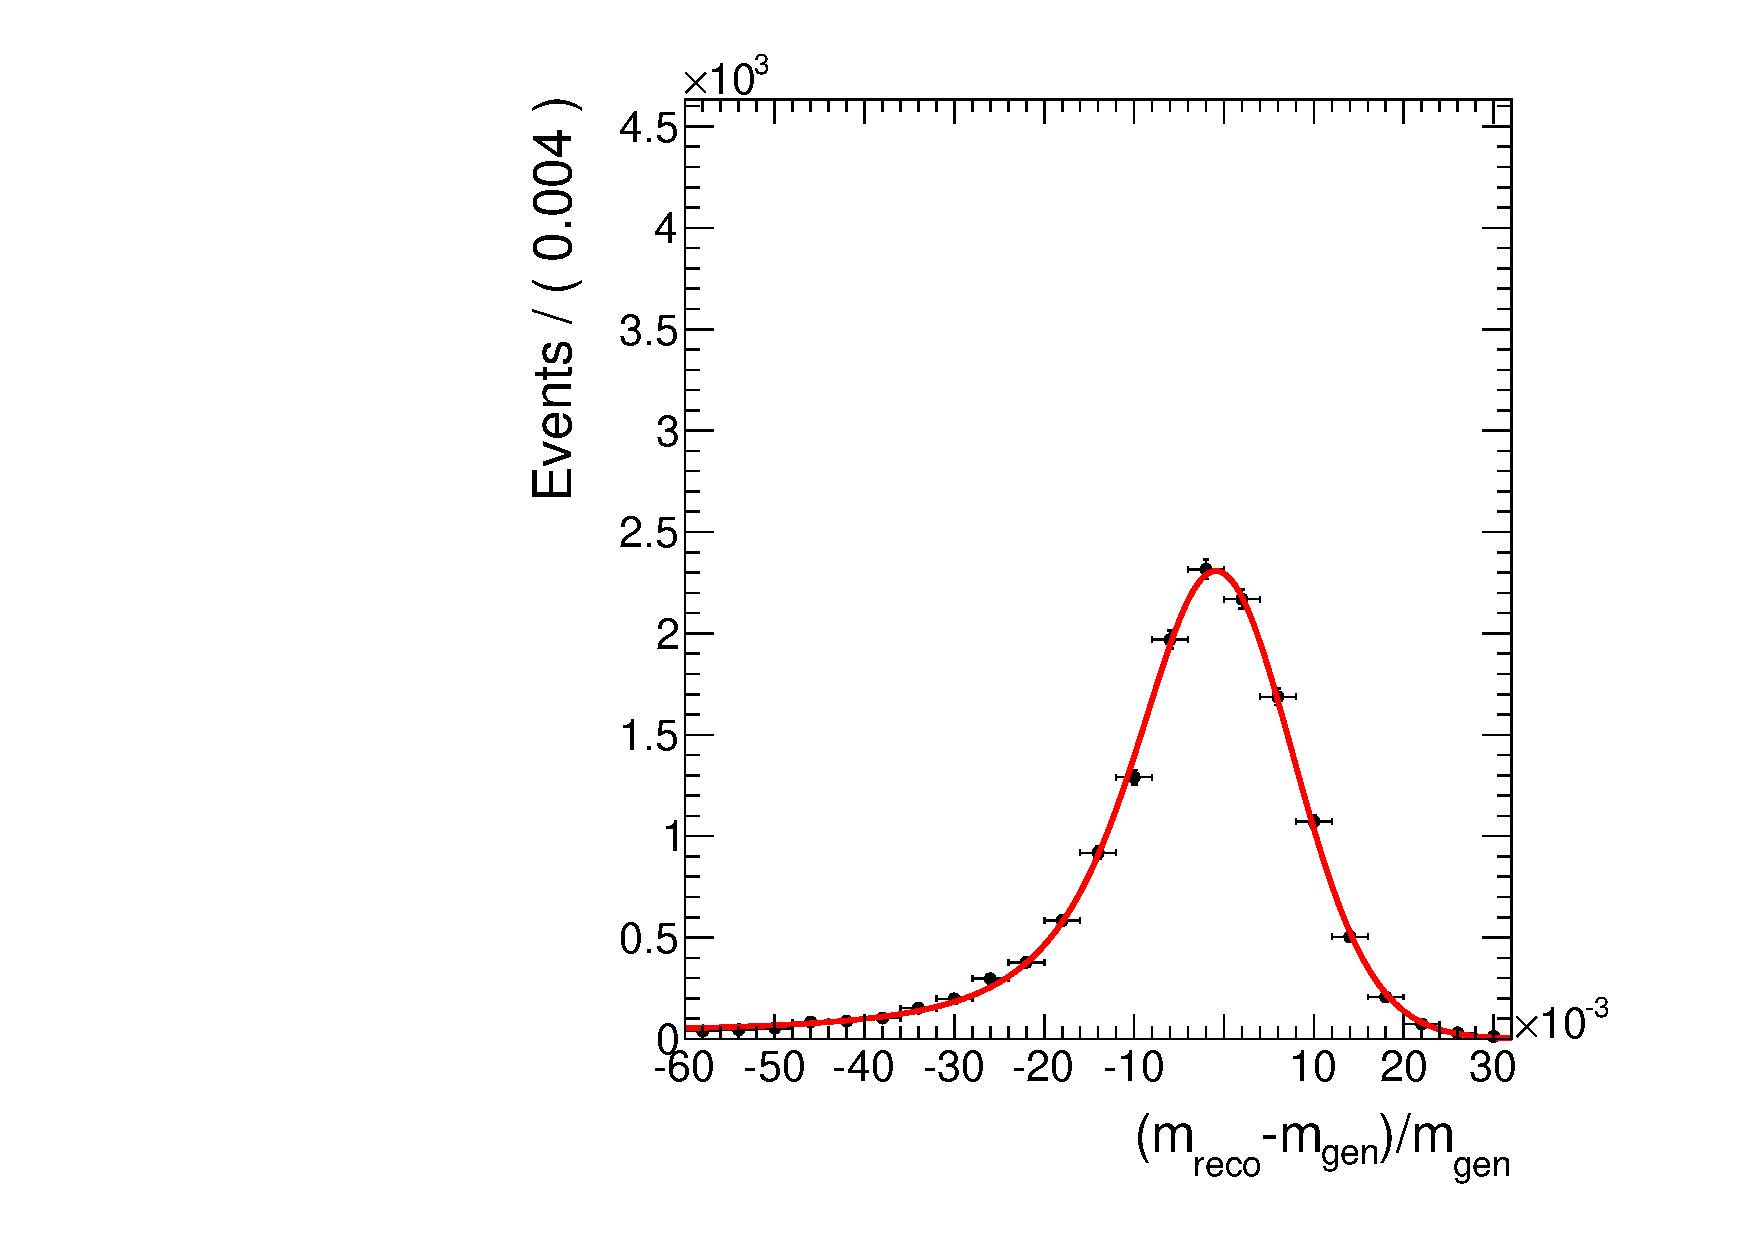
\includegraphics[width=0.22\textwidth]{fig/mass_resolution/Test_fit_results/resolution_BE/h_resolution_BE_7.pdf} &
%      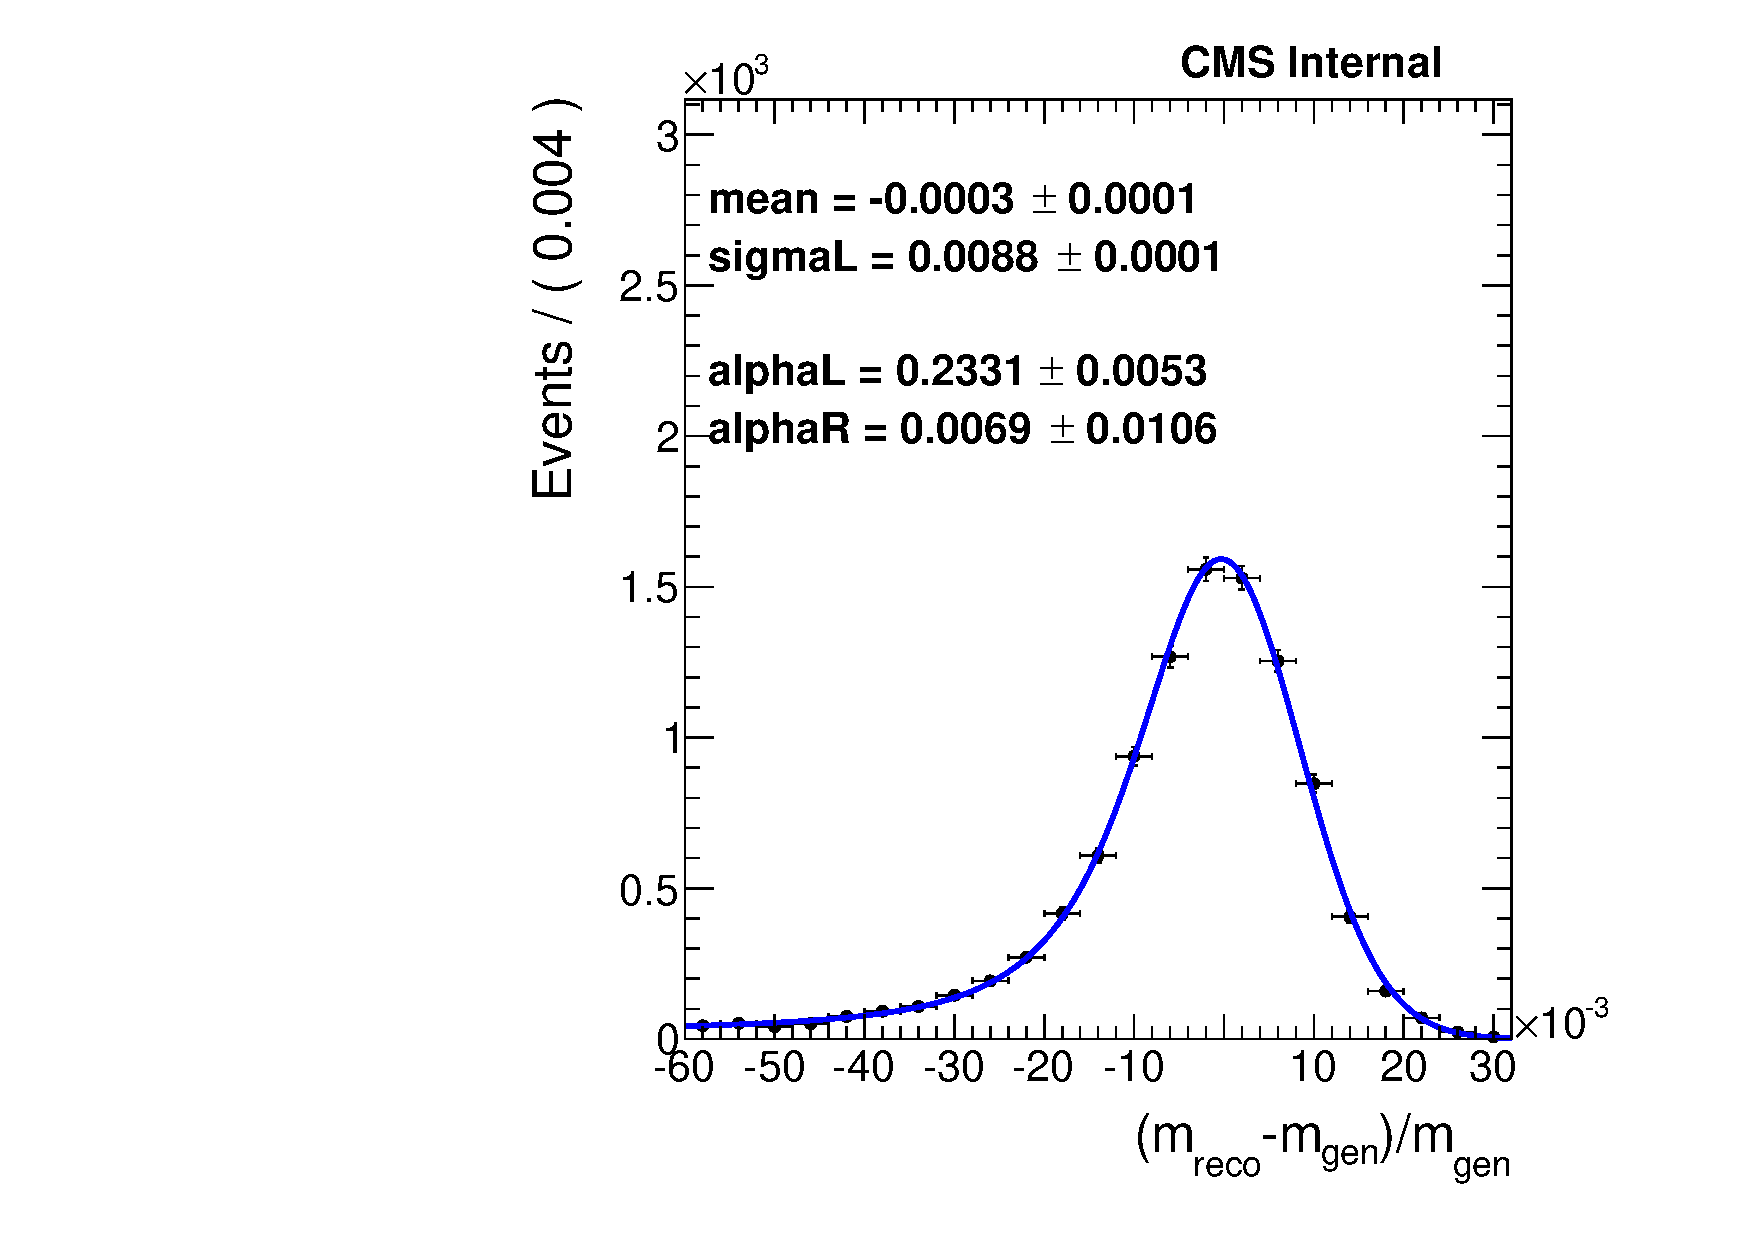
\includegraphics[width=0.22\textwidth]{fig/mass_resolution/Test_fit_results/resolution_BE/h_resolution_BE_8.pdf}\\
%    \end{tabular}
%    \caption{Closure test of the RC description in the BE category.
%    \label{fig:fit_closure_BE}}
%  \end{center}
%\end{figure}
